%% Antal Spector-Zabusky's UPenn thesis formatting skeleton, 2021
%%
%% Feel free to use any of this as necessary; you can contact me about it at
%% <antal.b.sz@gmail.com>.  This isn't all the styling in my thesis; it's mostly
%% limited to things that help you satisfy the formatting guidelines instead of
%% style choices.  It does not contain styling for things I didn't include, such
%% as a dedication or an index.  I wrote this for a CS thesis, so some details
%% may be specific to that.
%%
%% This should follow the formatting guidelines from
%% <https://guides.library.upenn.edu/dissertation_manual/formatting> as of
%% Spring 2021.
%%
%% Explanatory comments are annotated with ASZ; you can delete them if you
%% want.
%%
%% Good luck!

%% ASZ: 12 point font, single-sided (don't alternate left/right margins), and
%% sensible defaults.
\documentclass[12pt,oneside,reqno]{amsbook}

%%%%%%%%%%%%%%%%%%%%%%%%%%%%%%%%%%%%%%%%%%%%%%%%%%%%%%%%%%%%%%%%%%%%%%%%%%%%%%%%

%% ASZ: My usual "make things look nice and behave well" block
\usepackage[utf8]{inputenc}
\usepackage[T1]{fontenc}
\usepackage{lmodern}
\usepackage{microtype}
\usepackage{accsupp}
\usepackage{etoolbox}
\usepackage{newunicodechar}
\usepackage[dvipsnames,svgnames,x11names]{xcolor}
\usepackage{hyperref}
\usepackage{xspace}
\usepackage{advdate}
\usepackage[iso]{datetime}
\newdateformat{httpdate}{\shortdayofweekname{\THEDAY}{\THEMONTH}{\THEYEAR},~\THEDAY~\shortmonthname[\THEMONTH]~\THEYEAR}
\usepackage[
  backend=biber]{biblatex}
\addbibresource{bibliography.bib}

\usepackage{draft} % local
\newif\ifdraft\drafttrue
\newnote{lys}{BrickRed}
\newnote{bcp}{Chocolate}
\newnote{sz}{violet}
\newnote{ly}{orange}

\theoremstyle{definition}
\newtheorem{definition}{Definition}
\newtheorem{lemma}{Lemma}[chapter]

\def\chapterautorefname{Chapter}
\def\sectionautorefname{Section}
\def\subsectionautorefname{Subsection}
\def\subsubsectionautorefname{Subsubsection}
\def\lstnumberautorefname{Line}
\def\lemmaautorefname{Lemma}
\def\definitionautorefname{Definition}
\renewcommand{\equationautorefname}{Hypothesis}
\renewcommand{\itemautorefname}{Rule}
\usepackage{textcomp,listings,lstparams,lstcoq,graphicx,enumitem}
\lstdefinestyle{customcoq}{
  language=Coq,
  literate={<>}{$\ne$}1
  {->}{$\to$}1
  {<-}{$\gets$}1
  {=>}{$\Rightarrow$}1
  {|->}{$\mapsto$}1
  {fun}{$\lambda$}1
  {\\in}{$\in$}1
  {\\\/}{$\vee$}1
  {<>}{$\neq$}1
  {>>}{$\gg$}1
  {>>=}{$\gg\!=$}1
  {forall}{$\forall$}1
  {+'}{$\oplus$}1
  {sigma}{$\sigma$}1
}
\lstdefinestyle{json}{
  language=Coq,
  literate={@}{$@$}1
  {this}{$\ottkw{this}$}4
  {ref}{$\ottkw{ref}$}3
}
\lstdefinestyle{customc}{
  language=C,
  keywordstyle={\bfseries\codestyle\color{Keyword1Color}},
  showstringspaces=false,
  morekeywords={true,false,bool}
}
\newcommand{\http}{HTTP/1.1\xspace}
\newcommand{\inlinec}[1]{\lstinline[style=customc]{#1}}
\newcommand{\ilc}[1]{\lstinline[style=customcoq]{#1}}
\newcommand{\ilj}[1]{\lstinline[style=json]{#1}}
\lstnewenvironment{coq}{\lstset{style=customcoq}}{}
\lstnewenvironment{cpp}{\lstset{style=customc}}{}
\lstnewenvironment{json}{\lstset{style=json}}{}
\lstset{escapechar=\%,style=customcoq}

\usepackage{mathtools}
%% https://tex.stackexchange.com/a/127018
\usepackage{etoolbox}
\expandafter\patchcmd\csname \string\lstinline\endcsname{%
  \leavevmode
  \bgroup
}{%
  \leavevmode
  \ifmmode\hbox\fi
  \bgroup
}{}{%
  \typeout{Patching of \string\lstinline\space failed!}%
}

\usepackage{amssymb}
\newcommand{\complies}[2]{\mathsf{comply}_{#1}~{#2}}
\newcommand{\ncomplies}[2]{\neg(\complies{#1}{#2})}
\newcommand{\valid}[2]{\mathsf{valid}_{#1}~{#2}}
\newcommand{\invalid}[2]{\neg(\valid{#1}{#2})}
\newcommand{\accepts}[2]{\mathsf{accept}_{#1}~{#2}}
\newcommand{\rejects}[2]{\neg(\accepts{#1}{#2})}
\newcommand{\rejSound}[2]{#1\;\mathsf{sound}_{#2}^\mathfrak{Rej}}
\newcommand{\rejComplete}[2]{#1\;\mathsf{complete}_{#2}^\mathfrak{Rej}}
\newcommand{\exhaustive}[2]{\mathsf{exhaustive}_{#1}~{#2}}
\newcommand{\triggers}[3]{#1\overset{#3}\longrightarrow_{#2}}
\newcommand{\behaves}[2]{\triggers{#1}{}{#2}}
\newcommand{\llet}{\mathsf{let}\;}
\newcommand{\iin}{\mathsf{in}\;}
\newcommand{\letin}[2]{\llet#1=#2\;\iin}
\newcommand{\option}{\mathsf{option}\;}
\newcommand{\Some}[1]{\mathsf{Some}\;#1}
\newcommand{\None}{\mathsf{None}}
\newcommand{\sigT}[2]{\{\exists#1,#2\}}
\newcommand{\existT}[3]{\mathsf{pack}\;#1=#2\;\mathsf{with}\;#3}
\newcommand{\sstep}{\mathsf{sstep}}
\newcommand{\vstep}{\mathsf{vstep}}
\newcommand{\Server}{\mathsf{Server}}
\newcommand{\Validator}{\mathsf{Validator}}
\newcommand{\stepServer}{\mathsf{stepServer}}
\newcommand{\stepValidator}{\mathsf{stepValidator}}
\newcommand{\lam}[2]{\lambda#1\Rightarrow#2}
\newcommand{\Set}{\mathsf{set}\;}
\newcommand{\List}{\mathsf{list}\;}
\newcommand{\nil}{\varepsilon}
\newcommand{\If}{\mathsf{if}\;}
\newcommand{\tthen}{\mathsf{then}\;}
\newcommand{\Then}{\;\tthen}
\newcommand{\eelse}{\mathsf{else}\;}
\newcommand{\Else}{\;\eelse}
\newcommand{\Unit}{()}
\newcommand{\Tt}{()}
\newcommand{\Nat}{\mathbb N}
\newcommand{\Int}{\mathbb Z}
\newcommand{\Bool}{\mathbb B}
\newcommand{\True}{\mathsf{true}}
\newcommand{\False}{\mathsf{false}}
\newcommand{\Is}{\;\mathsf{is}\;}
\newcommand{\Prog}{\mathsf{Prog}}
\newcommand{\Lang}{\textsf{QAC-Lang}}
\newcommand{\serverOf}{\mathsf{serverOf}}
\newcommand{\validatorOf}{\mathsf{validatorOf}}
\newcommand{\Return}{\mathsf{return}}
\newcommand{\Sexp}{\mathsf{SExp}}
\newcommand{\Mem}{\mathsf{mem}}
\newcommand{\Exec}{\mathsf{exec}}
\newcommand{\update}[3]{#1[#2\mapsto#3]}
\newcommand{\constraint}{\mathsf{constraint}}
\newcommand{\Fresh}{\mathsf{fresh}\;}
\newcommand{\solvable}{\mathsf{solvable}\;}
\newcommand{\Vexp}{\mathsf{VExp}}
\newcommand{\oop}{\;op\;}
\newcommand{\ccmp}{\;cmp\;}
\newcommand{\Var}{\mathsf{var}}
\newcommand{\Reflects}[2]{#1\sim #2}
\newcommand{\satisfy}[2]{#1\;\mathsf{satisfy}\;#2}
\newcommand{\Jref}[3]{#1.#2.#3}
\newcommand{\Jpath}{\mathsf{Jpath}}
\newcommand{\This}{\mathsf{this}}
\newcommand{\Number}{\#}
\newcommand{\At}{@}
\newcommand{\Write}{\mathsf{write}}
\newcommand{\Havoc}{\mathsf{havoc}}

%% ASZ: `amsbook` didn't style `\paragraph`s appropriately
\patchcmd{\paragraph}{\normalfont}{\itshape}
  {} % Success
  {\GenericError
     {} % Continuation for \MessageBreak (unused)
     {Could not redefine \string\paragraph\space to be italic}
     {(This is a hack in the preamble.)} % Where to look for more info?
     {I tried to replace \string\normalfont\space with \string\itshape, but I
      couldn't.}}

%% ASZ: Change the spacing in the list of figures – I don't know if you need
%% this or not
\makeatletter
\patchcmd{\l@figure}{1.5pc}{2.25pc}
  {} % Success
  {\GenericError
     {} % Continuation for \MessageBreak (unused)
     {Could not fix the spacing in the list of figures}
     {(This is a hack in the preamble.)} % Where to look for more info?
     {I tried to replace the 1.5pc figure number--figure description separation
      with a 2.25pc separation in \string\l@figure\space, but I couldn't.}}

%% ASZ: I like it when tables of contents know where they are
\patchcmd{\@starttoc}{\ifx\contentsname}{\iffalse}
  {} % Success
  {\GenericError
     {} % Continuation for \MessageBreak (unused)
     {Could not add a line to the table of contents for itself}
     {(This is a hack in the preamble.)} % Where to look for more info?
     {I tried to replace the check in \string\@starttoc\space that suppresses a
      table of contents entry for the table of contents, but I couldn't.}}

%% ASZ: The other half of the above
\patchcmd{\@starttoc}{\@tocwrite}{\phantomsection\@tocwrite}
  {} % Success
  {\GenericError
     {} % Continuation for \MessageBreak (unused)
     {Could not add link targets to the table of contents/front matter lists}
     {(This is a hack in the preamble.)} % Where to look for more info?
     {I tried to add \string\phantomsection\space to \string\@starttoc\space so
      that it would generate hyperlink targets, but I couldn't.}}
\makeatother

%% ASZ: Set the page layout correctly: 1.5" margins on the left, 1" margins
%% everywhere else, page numbers count
\usepackage{fullpage}
\usepackage[margin=1in,left=1.5in,includeheadfoot]{geometry}

%% ASZ: Make footnote numbers run continuously, rather than restart at the start
%% of every chapter; this is required by the formatting guidelines
\counterwithout*{footnote}{chapter}

%% ASZ: I found these to be much clearer
\numberwithin{section}{chapter}
\numberwithin{figure}{chapter}
\numberwithin{equation}{chapter}
\numberwithin{definition}{chapter}

%%%%%%%%%%%%%%%%%%%%%%%%%%%%%%%%%%%%%%%%%%%%%%%%%%%%%%%%%%%%%%%%%%%%%%%%%%%%%%%%

%% ASZ: This is a package for generating and styling the various "preliminary
%% pages": title page, copyright page, and abstract
\usepackage{upenn-dissertation-preliminary-pages} % local
\NoSignatureLines %% ASZ: For COVID – turns off adding lines on the title page
                  %% for people to sign.  The default is \YesSignatureLines.
\SingleSpaceAbstract %% ASZ: I think it looks better than a double-spaced
                     %% abstract, although in deference to the guidelines,
                     %% \DoubleSpaceAbstract is the default.

%% ASZ: Fill out your own information here :-)  Some notes:
%%
%% * You need to specify your advisor, the graduate chair, and your committee
%%   members, even if there's overlap between these groups.
%%
%%   * Your external committee member(s) need both their title and their
%%   affiliation; below, just imagine that everyone but Gödel works at Penn.
%%
%% * Note that some of the faculty involved for you may be assistant or
%%   associate professors (but I couldn't bring myself to apply that title to
%%   any of these luminaries).  I don't believe extra titles (e.g., "ENIAC
%%   President's Distinguished Professor") are necessary.
%%
%% * Only one committee chair is supported; you'll need to modify
%%   `upenn-dissertation-preliminary-pages.sty` (or email me about it) to change
%%   that.
%%
%% * When rendering the title page, your chair (if present) comes first,
%%   followed by the rest of the committee in the same order as in the TeX.
%%
%% * Using a Creative Commons license is optional, and thus so is specifying
%%   `\creativecommons`.  If you want to use one, choose from the licenses
%%   available at <https://creativecommons.org/licenses/>, perhaps by using the
%%   license chooser at <https://creativecommons.org/choose/>.  You'll have to
%%   copy the name of the  license (including the short string) and the URL
%%   separately, as you can see with the text below (the license I used); I
%%   didn't build a LaTeX Creative Commons license parser (yet? :-)).
\title{Testing by Dualization}
\author{Yishuai Li}
\graduategroup{Computer and Information Science}
\graduationyear{2022}
\advisor{Benjamin C. Pierce}{Professor of Computer and Information Science}
\graduatechair{Mayur Naik}{Professor of Computer and Information Science}
\committeechair{Steve Zdancewic}{Professor of Computer and Information Science}
\committeemember{Mayur Naik}{Professor of Computer and Information Science}
\committeemember{Boon Thau Loo}{Professor of Computer and Information Science}
\committeemember{John Hughes}{Professor of Computing Science, Chalmers University of Technology}
\creativecommons
  {Attribution-Share\-Alike 4.0 International (CC BY-SA 4.0)}
  {https://creativecommons.org/licenses/by-sa/4.0/}

\begin{document}

%% ASZ: Roman page numbers
\frontmatter

\maketitle

\copyrightpage

\chapter*{Acknowledgments}
\label{chap:acknowledgments}

Lorem ipsum dolor sit amet, consectetur adipiscing elit, sed do eiusmod tempor
incididunt ut labore et dolore magna aliqua. Ut enim ad minim veniam, quis
nostrud exercitation ullamco laboris nisi ut aliquip ex ea commodo
consequat. Duis aute irure dolor in reprehenderit in voluptate velit esse cillum
dolore eu fugiat nulla pariatur. Excepteur sint occaecat cupidatat non proident,
sunt in culpa qui officia deserunt mollit anim id est laborum.

%% ASZ: ... the rest of your acknowledgments go here ...

%% ASZ: The `upenn-dissertation-preliminary-pages` package will correctly style
%% this, including your thesis name, your name, and your advisor's name.
\begin{abstract}{chap:abstract}
  Lorem ipsum dolor sit amet, consectetur adipiscing elit, sed do eiusmod tempor
  incididunt ut labore et dolore magna aliqua. Ut enim ad minim veniam, quis
  nostrud exercitation ullamco laboris nisi ut aliquip ex ea commodo
  consequat. Duis aute irure dolor in reprehenderit in voluptate velit esse
  cillum dolore eu fugiat nulla pariatur. Excepteur sint occaecat cupidatat non
  proident, sunt in culpa qui officia deserunt mollit anim id est laborum.
\end{abstract}

\tableofcontents
\listoffigures

%% ASZ: Arabic page numbers
\mainmatter

\chapter{Introduction}
\label{chap:introduction}
Software engineering requires rigorous testing of rapidly evolving programs,
which costs manpower comparable to developing the product itself.  To guarantee
programs' compliance with the specification, we need testers that can tell
compliant implementations from violating ones.

This thesis studies the testing of interactive systems' semantics: The system
under test (SUT) interacts with the tester by sending and receiving messages,
and the tester determines whether the messages sent by the SUT are valid or not
with respect to the protocol specification.

This chapter provides a brief view of interactive testing
(\autoref{sec:interactive-testing}), explains why nondeterminism makes this
problem difficult
(Sections~\ref{sec:internal-external-nondeterminism}--\ref{sec:inter-execution-nondeterminism}),
and discusses how language designs address the challenges caused by
nondeterminism (\autoref{sec:contribution}).

\section{Interactive Testing}
\label{sec:interactive-testing}
Suppose we want to test a web server that supports GET and PUT methods:
\begin{coq}
  CoFixpoint server (data: key -> value) :=
    request <- recv;;
    match request with
    | GET k   => send (data k);; server  data
    | PUT k v => send  Done   ;; server (data [k |-> v])
    end.
\end{coq}
We can write a tester client that interacts with the server and determines
whether it behaves correctly:
\begin{coq}
  CoFixpoint tester (data: key -> value) :=
    request <- random;;
    send request;;
    response <- recv;;
    match request with
    | GET k   => if response =? data k
                 then tester data
                 else reject
    | PUT k v => if response =? Done
                 then tester (data [k |-> v])
                 else reject
    end.
\end{coq}
This tester implements a reference server internally that computes the expected
behavior.  The behavior is then compared against that produced by the SUT.  The
tester rejects the SUT upon any difference from the computed expectation.

The above tester can be viewed as two modules: (i) a {\em test harness} that
interacts with the server and produces transactions of sends and receives, and
(ii) a {\em validator} that determines whether the transactions are valid or
not:
\begin{coq}
  (* Compute the expected response and next state of the server. *)
  Definition serverSpec request data :=
    match request with
    | GET k   => (data k, data)
    | PUT k v => (Done  , data [k |-> v])
    end.
  (* Validate the transaction against the stateful specification. *)
  Definition validate spec request response data :=
    let (expect, next) := spec request data in
    if response =? expect then Success next else Failure.
  (* Produce transactions for the validator. *)
  CoFixpoint harness validator state :=
    request <- random;;
    send request;;
    response <- recv;;
    if validator request response state is Success next
    then harness validator next
    else reject.
  Definition tester := harness (validate serverSpec).
\end{coq}
Such testing method works for deterministic systems, whose behavior can be
precisely computed from its input.  Whereas, many systems are allowed to behave
nondeterministically.  How to test systems that involve randomness?  How to
validate servers' behavior against concurrent clients?  The following sections
discuss nondeterminism by partitioning it in two ways, and explains how they
pose challenges to the validator and the test harness.

\section{Internal and external nondeterminism}
\label{sec:internal-external-nondeterminism}
When people talk to each other, voice is transmitted over substances.  When
testers interact with the SUT, messages are transmitted via the runtime
environment.  The specification might allow SUTs to behave differently from each
other, just like people speaking in different accents, we call it {\em internal
  nondeterminism}.  The runtime environment might affect the transmission of
messages, just like solids transmit voice faster than liquids and gases, we call
it {\em external nondeterminism}.

\subsection{Internal nondeterminism}
\label{sec:internal-nondeterminism}
Within the SUT, correct behavior may be \mbox{underspecified}.  For example,
HTTP~\cite{rfc7232} allows requests to be conditional: If the client has a local
copy of some resource and the copy on the server has not changed, then the
server needn't resend the resource.  To achieve this, an HTTP server may
generate a short string, called an ``entity tag'' (ETag), identifying the
content of some resource, and send it to the client:
\begin{center}
  \begin{minipage}[t]{.4\textwidth}
    \begin{cpp}
/* Client: */
GET /target HTTP/1.1
    \end{cpp}
  \end{minipage}\begin{minipage}[t]{.4\textwidth}
    \begin{cpp}
/* Server: */
HTTP/1.1 200 OK
ETag: "tag-foo"
... content of /target ...
    \end{cpp}
  \end{minipage}
\end{center}
The next time the client requests the same resource, it can include the ETag in
the GET request, informing the server not to send the content if its ETag still
matches:
\begin{center}
\begin{minipage}[t]{.4\textwidth}
\begin{cpp}
/* Client: */
GET /target HTTP/1.1
If-None-Match: "tag-foo"
\end{cpp}
\end{minipage}\begin{minipage}[t]{.4\textwidth}
\begin{cpp}
/* Server: */
HTTP/1.1 304 Not Modified
\end{cpp}
\end{minipage}
\end{center}
If the ETag does not match, the server responds with code 200 and the updated
content as usual.

Similarly, if a client wants to modify the server's resource atomically by
compare-and-swap, it can include the ETag in the PUT request as
\inlinec{If-Match} precondition, which instructs the server to only update the
content if its current ETag matches:
\begin{center}
  \begin{minipage}[t]{.4\textwidth}
    \begin{cpp}
/* Client: */
PUT /target HTTP/1.1
If-Match: "tag-foo"
... content (A) ...
    \end{cpp}
  \end{minipage}
  \begin{minipage}[t]{.4\textwidth}
    \begin{cpp}
/* Server: */
HTTP/1.1 204 No Content
    \end{cpp}
  \end{minipage}

  \begin{minipage}[t]{.4\textwidth}
    \begin{cpp}
/* Client: */
GET /target HTTP/1.1
    \end{cpp}
  \end{minipage}
  \begin{minipage}[t]{.4\textwidth}
    \begin{cpp}
/* Server: */
HTTP/1.1 200 OK
ETag: "tag-bar"
... content (A) ...
    \end{cpp}
  \end{minipage}
\end{center}
If the ETag does not match, then the server should not perform the requested
operation, and should reject with code 412:
\begin{center}
  \begin{minipage}[t]{.4\textwidth}
    \begin{cpp}
/* Client: */
PUT /target HTTP/1.1
If-Match: "tag-baz"
... content (B) ...
    \end{cpp}
  \end{minipage}
  \begin{minipage}[t]{.4\textwidth}
    \begin{cpp}
/* Server: */
HTTP/1.1 412 Precondition Failed
    \end{cpp}
  \end{minipage}

  \begin{minipage}[t]{.4\textwidth}
    \begin{cpp}
/* Client: */
GET /target HTTP/1.1
    \end{cpp}
  \end{minipage}
  \begin{minipage}[t]{.4\textwidth}
    \begin{cpp}
/* Server: */
HTTP/1.1 200 ok
ETag: "tag-bar"
... content (A) ...
    \end{cpp}
  \end{minipage}
\end{center}
Whether a server's response should be judged {\em valid} or not depends on the
ETag it generated when creating the resource.  If the tester doesn't know the
server's internal state ({\it e.g.}, before receiving any 200 response that
includes an ETag), and cannot enumerate all of them (as ETags can be arbitrary
strings), then it needs to maintain a space of all possible values, and narrow
the space upon further interactions with the server.  For example, ``If the
server has revealed some resource's ETag as \inlinec{"tag-foo"}, then it must
not reject requests targetting this resource conditioned over \inlinec{If-Match:
  "tag-foo"}, until the resource has been modified''; and ``Had the server
previously rejected an \inlinec{If-Match} request, it must reject the same
request until its target has been modified.''

\begin{figure}
\begin{coq}
  Definition validate request response
             (data      : key -> value)
             (tag_is    : key -> Maybe etag)
             (tag_is_not: key -> list etag) :=
    match request, response with
    | PUT k t v, NoContent => 
      if t \in tag_is_not k then Failure
      else if (tag_is k =? Unknown) || strong_match (tag_is k) t
      then (* Now the tester knows that the data in [k]
            * is updated to [v], but its new ETag is unknown. *)
        Success (data       [k |-> v],
                 tag_is     [k |-> Unknown],
                 tag_is_not [k |-> [] ])
      else Failure
    | PUT k t v, PreconditionFailed =>
      if strong_match (tag_is k) t then Failure
      else (* Now the tester knows that the ETag of [k]
            * is other than [t]. *)
        Success (data, tag_is, tag_is_not [k |-> t::(tag_is_not k)])
    | GET k t, NotModified =>
      if t \in tag_is_not then Failure
      else if (tag_is k =? Unknown) || weak_match (tag_is k) t
      then (* Now the tester knows that the ETag of [k]
            * is equal to [t]. *)
        Success (data, tag_is [k |-> Known t], tag_is_not)
      else Failure
    | GET k t0, OK t v =>
      if weak_match (tag_is k) t0 then Failure
      else if data k =? v
      then (* Now the tester knows the ETag of [k]. *)
        Success (data, tag_is [k |-> Known t], tag_is_not)
      else Failure
    | _, _ => Failure
    end.
\end{coq}
  \caption[Ad hoc tester for \http conditional requests.]{Ad hoc tester for
    \http conditional requests.  \ilc{PUT k t v} represents a PUT request that
    changes \ilc k's value into \ilc v only if its ETag matches \ilc t; \ilc{GET
      k t} is a GET request for \ilc k's value only if its ETag does not match
    \ilc t; \ilc{OK t v} indicates that the request target's value is \ilc v and
    its ETag is \ilc t.}
  \label{fig:etag-tester}
\end{figure}

This idea of remembering matched and mismatched ETags is implemented in
\autoref{fig:etag-tester}.  For each key, the validator maintains three internal
states: (i) The value stored in \ilc{data}, (ii) the corresponding resource's
ETag, if known by the tester, stored in \ilc{tag_is}, and (iii) ETags that
should not match with the resource's, stored in \ilc{tag_is_not}.  Each pair of
request and response contributes to the validator's knowledge of the target
resource.  The tester rejects the SUT if the observed behavior does not match
its knowledge gained in previous interactions.

Even a simple nondeterminism like ETags requires such careful design of the
validator, based on thorough comprehension of the specification.  For more
complex protocols, we hope to construct the validator in a reasonable way.

\subsection{External nondeterminism}
\label{sec:intro-external-nondet}
To discuss the nondeterminism caused by the environment, we need to define the
environment concept in testing scenario.
\begin{definition}[Environment, input, output, and observations]
  {\em Environment} is the substance that the tester and the SUT interact with.
  {\em Input} is the subset of the environment that the tester can manipulate.
  {\em Output} is the subset of the environment that the SUT can alter.  {\em
    Observation} is the tester's view of the environment.
\end{definition}
When testing servers, the environment is the network stack between the client
and the server.  The input is the request sent by the client, and the output is
the response sent by the server.  The response is transmitted via the network,
until reaching the client side as observations.

\begin{figure}
  \centering
  \begin{minipage}[c]{.3\textwidth}
\begin{coq}
  (* Observation: *)
  1> PUT k "new"
  1< Done
  2> GET k
  2< "new"
\end{coq}
  \end{minipage}\begin{minipage}[c]{.4\textwidth}
  \includegraphics[width=\linewidth]{figures/linear-trace}
  \end{minipage}\begin{minipage}[c]{.3\textwidth}
\begin{coq}
  (* Output: *)
  1> PUT k "new"
  1< Done
  2> GET k
  2< "new"
\end{coq}
  \end{minipage}
  \caption[Linear trace upon no concurrency.]{Upon no concurrency, the
    observation is identical to the output.}
  \label{fig:linear-trace}
\end{figure}
\begin{figure}
  \centering
  \begin{minipage}[c]{.3\textwidth}
\begin{coq}
  (* Observation: *)
  1> PUT k "new"
  2> GET k
  1< Done
  2< "old"
\end{coq}
  \end{minipage}\begin{minipage}[c]{.4\textwidth}
    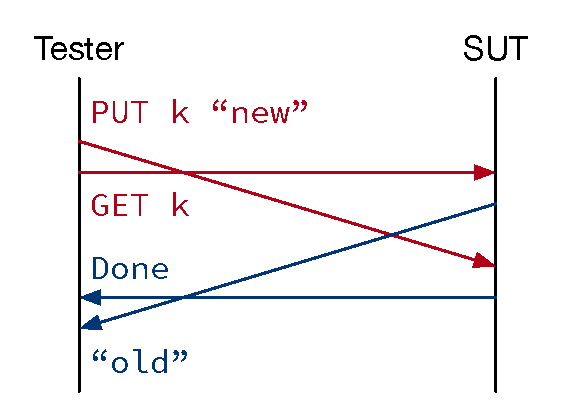
\includegraphics[width=\linewidth]{figures/network-trace}
  \end{minipage}\begin{minipage}[c]{.3\textwidth}
\begin{coq}
  (* Output: *)
  2> GET k
  2< "old"
  1> PUT k "new"
  1< Done
\end{coq}
  \end{minipage}
  \caption[Reordered trace upon network delays.]{Acceptable: The observation can
    be explained by a valid output reordered by the network environment.}
  \label{fig:reordered-trace}
\end{figure}
\begin{figure}
  \centering
  \begin{minipage}[c]{.3\textwidth}
\begin{coq}
  (* Observation: *)
  1> PUT k "new"
  1< Done
  2> GET k
  2< "old"
\end{coq}
  \end{minipage}\begin{minipage}[c]{.4\textwidth}
  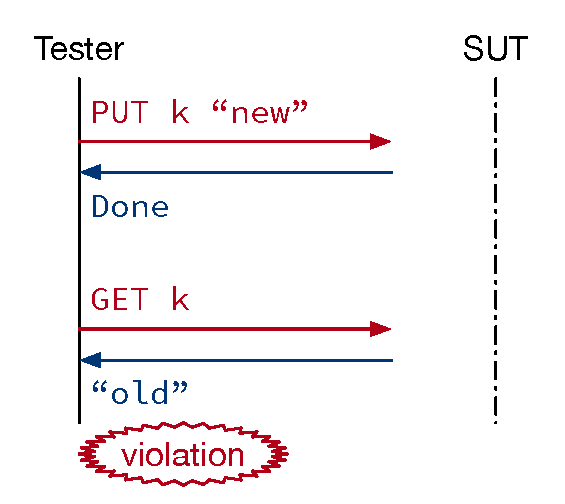
\includegraphics[width=\linewidth]{figures/invalid-trace}
  \end{minipage}\begin{minipage}[c]{.3\textwidth}\
  \end{minipage}
  \caption[Invalid trace that violates the specification.]{Unacceptable: The
    tester received the \ilc{Done} response before sending the \ilc{GET}
    request, thus the SUT must have processed the \ilc{PUT} request before the
    \ilc{GET} request.  Therefore, the \ilc{"old"} response must be invalid.}
  \label{fig:invalid-trace}
\end{figure}
The tester shown in \autoref{sec:interactive-testing} runs one client at a time.
It waits for the response before sending the next request, as shown in
\autoref{fig:linear-trace}.  Such tester's observation is guaranteed identical
to the SUT's output, so it only needs to scan the requests and responses with
one stateful validator.

To reveal the server's behavior upon concurrent requests, the tester needs to
simulate multiple clients, sending new requests before receiving previous
responses.  The network delay might cause the server to receive requests in a
different order from that on the tester side.  Vice versa, responses sent by the
server might be reordered before arriving at the tester, as shown in
\autoref{fig:reordered-trace}.  Such tester's observation can be explained by
various outputs on the SUT side.  The validator needs to consider all possible
outputs that can explain such observation, and see if anyone of them complies
with the specification.  If no valid output can explain the observation, then
the tester should reject the SUT, as shown in \autoref{fig:invalid-trace}.

We hope to construct a tester that can handle external nondeterminism
systematically, and provide a generic way for reasoning on the environment.

\section{Test harness and inter-execution nondeterminism}
\label{sec:inter-execution-nondeterminism}
A good tester consists of (i) a validator that accurately determines whether its
observations are valid or not, and (ii) a test harness that can reveal invalid
observations effectively.  \autoref{sec:internal-external-nondeterminism} has
explained the challenges in the validator.  Here we discuss the test harness.

\subsection{Test harness}
Intuitively, a tester generates test input and executes the test.  It then
validates the observation and accepts/rejects the SUT, as shown in
\autoref{fig:gen-only}.
\begin{figure}
  \includegraphics[width=.5\linewidth]{figures/gen-only}
  \caption{Simple tester architecture without shrinking.}
  \label{fig:gen-only}
\end{figure}

However, to achieve better coverage, a randomized generator might produce huge
test input.  Suppose the tester has revealed invalid observation after thousands
of interactions, such report provides limited intuition of where the bug was
introduced.  To help developers locate the bug more effectively, the tester
should present a {\em minimal counterexample} that can reproduce the violation.
This is done by {\em shrinking} the failing input and rerunning the test with
the input's substructures.  As shown in \autoref{fig:gen-shrink}, if a test
input has no substructure that can cause any failure, then we report it as the
minimal counterexample.
\begin{figure}
  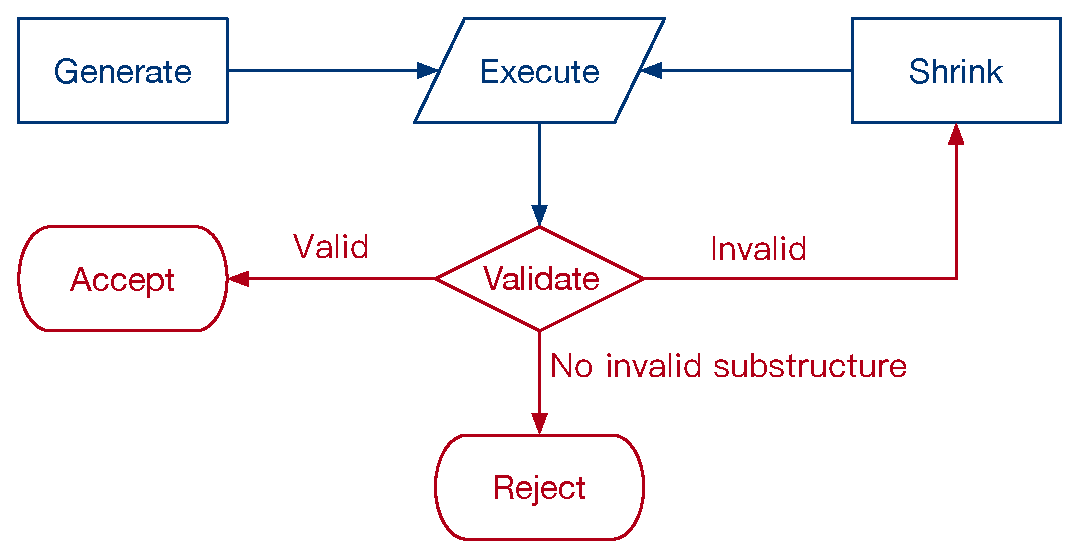
\includegraphics[width=.8\linewidth]{figures/gen-shrink}
  \caption{Tester architecture with shrinking mechanism.}
  \label{fig:gen-shrink}
\end{figure}

The test harness consists of generator, shrinker, and executor.  This thesis
studies the generator and the shrinker that produce the test input.  The
executor that produces observations based on the input is discussed in the
related works chapter.

Interesting test inputs are those that are more likely to reveal invalid
observations.  Such subset is usually sparse and cannot be enumerated within
reasonable budget {\it e.g.} in \autoref{sec:internal-nondeterminism}, request
ETags that match the target resources'.  The tester needs to manipulate the
inputs' distribution, by implementing heuristics that emphasize certain input
patterns.  Such heuristics is challenged by another form of nondeterminism
discussed as follows.

\subsection{Inter-execution nondeterminism}
Consider \http, where requests may be conditioned over timestamps.  If a client
has cached a version with a certain timestamp, then it can send the timestamp as
\inlinec{If-Modified-Since} precondition.  The server should not transmit the
request target's content if its \inlinec{Last-Modified} timestamp is not newer
than the precondition's:
\begin{cpp}[escapeinside={(*}{*)}]
  /* Client: */
  GET /index.html HTTP/1.1
  If-Modified-Since: (*\httpdate\DayAfter[-1]~\currenttime *) GMT
                             /* Server: */
                             HTTP/1.1 200 OK
                             Last-Modified: (*\httpdate\today~\currenttime *) GMT
                             ... content of target ...
  /* Client: */
  GET /index.html HTTP/1.1
  If-Modified-Since: (*\httpdate\today~\currenttime *) GMT
                             /* Server: */
                             HTTP/1.1 304 Not Modified
\end{cpp}
In this scenario, an interesting candidate for the \inlinec{If-Modified-Since}
precondition is the \inlinec{Last-Modified} timestamp of a previous response.
To emphasize this request pattern, the tester needs to implement heuristics that
generates test inputs based on previous observations.

In case the tester has revealed invalid observations from the server, it needs
to rerun the test with shrunk input.  The timestamps on the server might be
different from the previous execution, so an interesting timestamp in a previous
run might become trivial in this run.

Such inter-execution nondeterminism poses challenges to the input minimization
process: To preserve the input pattern, the shrunk \http request should use the
timestamps from the new execution.  We hope to implement a generic shrinking
mechanism that can reproduce the heuristics in the test generator's design.

\section{Contribution}
\label{sec:contribution}
This thesis addresses the challenges in testing caused by various forms of
nondeterminism.  I introduce symbolic languages for specifying the protocol and
representing test input, and {\em dualize} the specification into the tester's
(1) validator, (2) generator, and (3) shrinker:

\begin{enumerate}
\item The specification is written as a reference implementation---a
  nondeterministic program that exhibits all possible behavior allowed by the
  protocol.  Internal and external nondeterminism are represented by symbolic
  variables, and the space of nondeterministic behavior is defined by all
  possible assignments of the variables.

  For internal nondeterminism, the validator computes the symbolic
  representation of the SUT's output.  The symbolic output expectation is then
  {\em unified} against the tester's observations, reducing the protocol
  compliance problem into constraint solving.

  For external nondeterminism, I introduce a model that specifies the
  environment.  The environment model describes the relation between the SUT's
  output and the tester's observations.  By composing the environment model with
  the reference implementation, we get a tester-side specification that defines
  the space of valid observations.
\item Test generation heuristics are defined as computations from observations
  to the next input.  To specify such heuristics in a generic way, I introduce
  intermediate representations for observations and test inputs, which are
  protocol-independent.

  Heuristics in this framework produces symbolic test inputs that are
  parameterized over observations.  During execution, the test harness computes
  the concrete input by {\em instantiating} the symbolic input's arguments with
  runtime observations.
\item The language for test inputs is designed with inter-execution
  nondeterminism in mind.  By instantiating the inputs' symbolic intermediate
  representation with different observations, the test harness gets different
  test inputs but preserves the pattern.

  To minimize counterexamples, the test harness only needs to shrink the inputs'
  symbolic representation.  When rerunning the test, the shrunk input is
  reinstantiated with the new observations, thus reproduces the heuristics by
  the test generator.
\end{enumerate}

\subsection*{Thesis claim}
Symbolic abstract representation can address challenges in testing interactive
systems with uncertain behavior.  Specifying protocols with symbolic reference
implementation enables validating observations of systems with internal and
external nondeterminism.  Representing test input and observations symbolically
allows generating and shrinking interesting test cases despite inter-execution
nondeterminism.  Combining these methods result in a rigorous tester that can
capture protocol violations effectively.

This claim is supported by the following publications:
\begin{enumerate}
\item {\it From C to Interaction Trees: Specifying, Verifying, and Testing a
  Networked Server}~\cite{cpp19}, with Nicolas Koh, Yao Li, Li-yao Xia, Lennart
  Beringer, Wolf Honor\'e, and William Mansky, where I developed a tester
  program based on a swap server's specification written as ITrees~\cite{itree},
  and evaluated the tester's effectiveness by mutation testing.
\item {\it Verifying an HTTP Key-Value Server with Interaction Trees and
  VST}~\cite{itp21}, with Hengchu Zhang, Wolf Honor\'e, Nicolas Koh, Yao Li,
  Li-yao Xia, Lennart Beringer, and William Mansky, where I developed the
  top-level specification for \http, and derived a tester client that revealed
  liveness and interrupt-handling bugs in our HTTP server, despite it was
  formally verified.
\item {\it Model-Based Testing of Networked Applications}~\cite{issta21}, which
  describes my technique of specifying \http with symbolic reference
  implementations, and from the specification, automatically deriving a tester
  program that can find bugs in Apache and Nginx.
\item {\it Testing by Dualization} (to be submitted to OOPSLA), a theory for
  interactive testing, explaining how to specify protocols using abstract model
  implementations, and how to guarantee the soundness and completeness of
  validators derived from the abstract model.
\end{enumerate}

\subsection*{Outline}
This thesis is structured as follows:


\chapter{Dualization Theory}
\label{chap:theory}
During the testing practice in \autoref{chap:practices}, the tester's quality was
evaluated by mutation testing, {\it i.e.} running the tester against buggy
implementations to see if it rejects.  To formally prove that the tester is
good, I develop a theory for reasoning on testers' good properties.

{\em Interactive testing} is a process that reveals the SUT's interactions and
determines whether it satisfies the specification.  There are two kinds of
interactions: (1) {\em inputs} that the tester can specify, and (2) {\em
  outputs} that are observed from the SUT.  In particular, when testing
networked systems, the input is a message sent by the tester, and the output is
a message received from the SUT.

When viewing the SUT as a function from inputs to outputs, we can test the
system by (1) providing an input, (2) get the output, and (3) validating the
input-output pair.  This process is called {\em synchronous testing}.

However, the nature of networked systems is that multiple messages might arrive
at the system simultaneously, and a high-throughput system should handle the
messages concurrently.  To check the system's validity upon concurrent inputs,
the tester should send multiple messages, rather than executing ``one client at
a time''.  This non-blocking process is called {\em asynchronous testing}.

My goal is to formalise the techniques in \textcite{issta21} into a generic
theory for asynchronous testing.

A tester consists of two parts: (i) a test harness that interacts with the SUT
and observes the interactions, and (ii) a validator that determines whether the
observations satisfy the specification.

The test harness needs to produce counterexamples effectively, and provide good
coverage of test cases.  The goal is to locate unknown bugs within a fixed
budget, which is more practical than theoretical, and will be discussed in
\autoref{sec:harness}.  The test theory in this dissertation focuses on
guaranteeing the soundness and completeness of the validator logic.

Testers are programs that determine whether implementations are compliant or
not, based on its observations.  This section defines the basic concepts and
notations in interactive testing.

\begin{definition}[Implementations and Traces]
  {\em Implementations} are programs that can interact with their environment.
  {\em Traces} are the implementations' inputs and outputs during execution.
  ``Implementation $i$ can {\em produce} trace $t$'' is written as ``$\behaves i
  t$''.
\end{definition}

This chapter focuses on synchronous testing that assumes no external
nondeterminism.  Here the tester's observation is identical to the
implementation's output, so the tester-side trace is the same as that on the
implementation side.  Asynchronous testing will be discussed in
\autoref{chap:practices}.

\begin{definition}[Specification, Validity, and Compliance]
  \label{def:compliance}
  A {\em specification} is a description of valid traces.  ``Trace $t$ is {\em
    valid} per specification $s$'' is written as ``$\valid s t$''.

  An implementation $i$ {\em complies} with a specification $s$ (written as
  ``$\complies s i$'') if it only produces traces that are valid per the
  specification:
  \[\complies s i\quad\triangleq\quad\forall t,(\behaves i t)\implies\valid s t\]
\end{definition}

\begin{definition}[Tester components and correctness]
  \label{def:tester}
  A tester consists of (i) a {\em validator} that accepts or rejects
  traces (written as ``$\accepts v t$'' and ``$\rejects v t$''), and
  (ii) a {\em test harness} that triggers different traces with
  various inputs.

  A tester is {\em correct} if its acceptances and rejections are sound and
  complete.  A tester is {\em rejection-sound} if it only rejects non-compliant
  implementations; it is {\em rejection-complete} if it can reject all
  non-compliant implementations, provided sufficient time of
  execution.\footnote{The semantics of ``soundness'' and ``completeness'' vary
    among contexts.  This thesis inherits terminologies from existing
    literature~\cite{Tretmans}, but explicitly uses ``rejection-'' prefix for
    clarity.  ``Rejection soundness'' is equivalent to ``acceptance
    completeness'', and vice versa.}
\end{definition}

The tester's correctness is based on its components' properties: A
rejection-sound tester requires its validator to be rejection-sound; A
rejection-complete tester consists of (i) a rejection-complete validator and
(ii) an exhaustive test harness that can eventually trigger invalid traces.  The
validators' soundness and completeness are defined as follows:

\begin{definition}[Correctness of validators]
  A validator $v$ is {\em rejection-sound} with respect to specification $s$
  (written as ``$\rejSound v s$'') if it only rejects traces that are invalid
  per $s$:
  \[\rejSound v s\quad\triangleq\quad\forall t,\rejects v t\implies\invalid s t\]

  A validator $v$ is {\em rejection-complete} with respect to specification $s$
  (written as ``$\rejComplete v s$'') if it rejects all behaviors that are
  invalid per $s$:
  \[\rejComplete v s\quad\triangleq\quad\forall t,\invalid s t\implies\rejects v t\]
\end{definition}

The rest of this chapter shows how to construct specifications and validators,
and how to prove the validators' correctness with respect to the specifications.



\chapter{Testing in Practice}
\label{chap:practices}
In \autoref{chap:theory}, I introduced the theory of validators using the QAC
language family.  I also shown how to prove validators' correctness with a
simple $\Prog$ language.

However, in real-world testing practices, there are more problems to consider.
For example: How to interact with the SUT via multiple channels?  How to handle
external nondeterminism?

\begin{figure}
  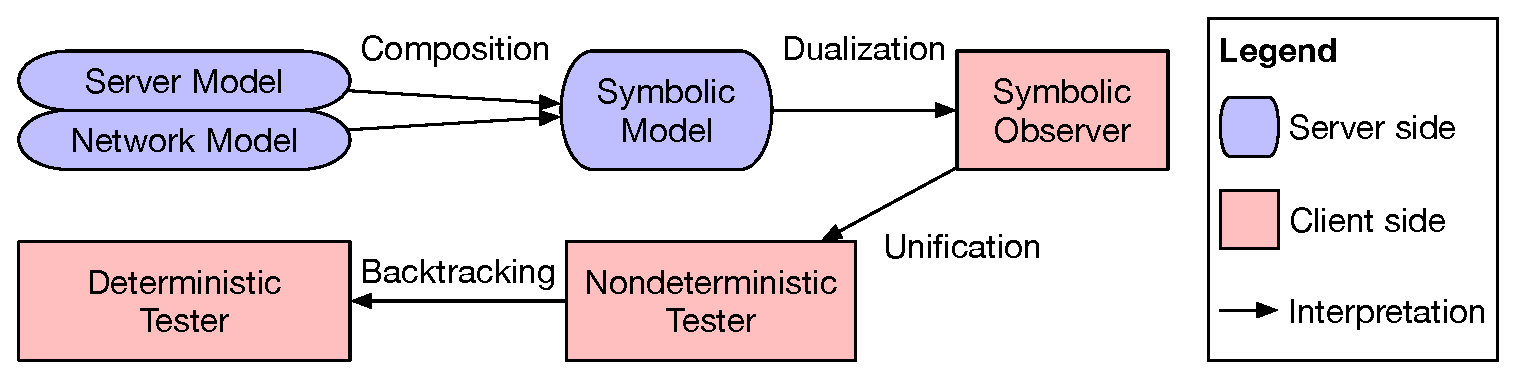
\includegraphics[width=\linewidth]{figures/framework}
  \caption{Deriving tester program from specification}
  \label{fig:framework}
\end{figure}

This chapter describes how to derive specifications into tester programs that
can interact with the SUT and reveal potential defects, using \http as an
example.  The derivation framework is shown in outline in
\autoref{fig:framework}.  Each box is a model program, and the arrows are
``interpretors'' that transform one model into another.

\autoref{sec:itree} introduces the ITree modelling language for specifying
protocols and deriving them into testers.  \autoref{sec:external-nondet} and
\autoref{sec:internal-nondet} address external and internal nondeterminism in
the ITree context.  \autoref{sec:backtrack} explains how to execute the derived
tester model as an interactive program.

\section{ITree Specification Language}
\label{sec:itree}
To write specifications for protocols' rich semantics, I employed ``interaction
tree'' (ITree), a generic data structure for representing interactive programs
in the Coq programming language, introduced by \citet{itree}.  ITrees allow
specifying protocols as monadic programs that model valid implementations'
possible behavior.  The ITree specification can be interpreted into a tester
program, as discussed in later sections.

\subsection{Language definition}
\label{sec:itree-lang}
Consider an echo program, which keeps reading some data and writing it out
verbatim, until reaching EOF.  We can represent the program in Coq, with a
reference in C as:
\begin{multicols}{2}
\begin{coq}
  CoFixpoint echo :=
    c <- getchar;;
    if c is EOF
    then EXIT
    else
      putchar c;;
      echo.
\end{coq}
\columnbreak
\begin{cpp}
  void echo() {
    const char c = getchar();
    if (c == EOF)
      return;
    else {
      putchar(c);
      echo();
    }
\end{cpp}
\end{multicols}
Here the behavior after \ilc{getchar} depends on the value actually read.  The
monadic computation in Coq can be desugared into:
\begin{coq}
  CoFixpoint echo :=
    Bind getchar
         (fun c => if c is EOF
                 then EXIT
                 else Bind (putchar c)
                           (fun _ => echo)
         ).
\end{coq}
Such continuation-passing style can be represented as a tree of interactions.
To help readers better understand the interaction tree language, I first provide
a modified version of it that better shows its tree structure, and then explain
the actual type definition used in practice.

\begin{figure}
\begin{coq}
  CoInductive itreeM (E: Type -> Type) (R: Type) :=
    Ret     : R   -> itreeM E R
  | Trigger : E R -> itreeM E R
  | Bind    : forall {X : Type}, itreeM E X -> (X -> itreeM E R) -> itreeM E R.
\end{coq}
\caption{Mock definition of interaction trees.}
\label{fig:mock-itree}
\end{figure}

\begin{figure}
  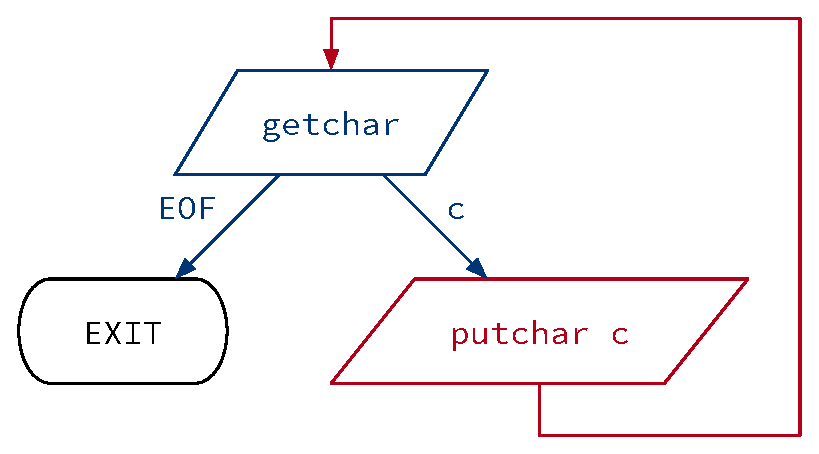
\includegraphics[width=.5\linewidth]{figures/echo-itree}
  \caption{Interaction tree for echo program}
  \label{fig:echo-itree}
\end{figure}

\paragraph{Mock interaction trees}
As shown in \autoref{fig:mock-itree}, a mock interaction tree (\ilc{itreeM}) has
two kinds of leaves, \ilc{Ret} and \ilc{Trigger}, and has internal nodes
constructed by \ilc{Bind}:
\begin{itemize}
\item \ilc{(Ret r)} represents a pure computation that yields a value \ilc r.
  In the echo example, \ilc{EXIT} halts the program with return value zero:
\begin{coq}
  Definition EXIT := Ret 0.
\end{coq}

\item \ilc{(Trigger e)} performs an impure event \ilc e and returns its result.
  Here \ilc{(e: E R)} is an event whose result is of type \ilc R.  For example,
  \ilc{getchar} has result type \ilc{char}, and \ilc{putchar}'s result type is
  \ilc{unit} (which corresponds to \inlinec{void} in C/C++, or \ilc{()} in
  Haskell).  These effective programs are constructed by triggering standard I/O
  events:
\begin{coq}
  Variant stdioE: Type -> Type := (* event type *)
    GetChar:         stdioE char
  | PutChar: char -> stdioE unit.
  
  Definition getchar           : itreeM stdioE char := Trigger  GetChar.
  Definition putchar (c: char) : itreeM stdioE unit := Trigger (PutChar c).
\end{coq}
\item \ilc{(Bind m k)} binds the return value of \ilc m to the continuation
  function \ilc k.  It first runs program \ilc m until it returns some value of
  type \ilc X.  The return value \ilc{(x: X)} then instantiates \ilc k into the
  following computation \ilc{(k x: itreeM E R)}.  This corresponds to the
  monadic \ilc{(;;)} syntax:
\begin{coq}
  Notation "x <- m1;; m2" := (Bind m1 (fun x => m2)).
  Notation "m1;; m2"      := (Bind m1 (fun _ => m2)).
\end{coq}

As illustrated in \autoref{fig:echo-itree}, each possible return value \ilc x is
an edge that leads to the child it instantiates, {\it i.e.}, \ilc{(k x)}.  In this
way, the \ilc{Ret} and \ilc{Trigger} nodes are connected into a tree
structure.
\end{itemize}

The mock interaction tree provides an intuitive continuation-passing structure
for representing impure programs.  However, to implement dualization
effectively, we need to revise the language definition of monadic binding.

\paragraph{Practical interaction trees}

\begin{figure}
\begin{coq}
  CoInductive itree (E: Type -> Type) (R: Type) :=
    Pure   : R -> itree E R
  | Impure : forall {X : Type}, E X -> (X -> itree E R) -> itree E R.
\end{coq}
\caption{Formal definition of interaction trees (simplified)}
\label{fig:itrees}
\end{figure}

Instead of binding a program to a continuation, ITree binds a single impure
event, as shown in \autoref{fig:itrees}.  I use \ilc{(Impure e k)} to
replace \ilc{(Bind (Trigger e) k)} representations in \ilc{itreeM}.
A \ilc{Pure} computation cannot be bound to a continuation, and must be the leaf
of an ITree.\footnote{For readability, the ``practical'' ITree definition is a
simplified version from \citet{itree}.  Here \ilc{Pure} and \ilc{Impure}
correspond to the \ilc{Ret} and \ilc{Vis} constructors.  I dropped the \ilc{(Tau
: itree E R -> itree E R)} constructor, which carries no semantics and is used
for satisfying Coq's guardedness condition.}

The \ilc{Ret}, \ilc{Trigger}, and \ilc{Bind} constructors introduced in
\ilc{itreeM} have equivalent representations in \ilc{itree}, so we can still
write programs in the monadic syntax:
\begin{coq}
  Definition ret {E R} : R -> itree E R := Pure.
  
  Definition trigger {E R} (e: E R) : itree E R := Impure e Pure.

  CoFixpoint bind {X E R} (m: itree E X) (f: X -> itree E R) : itree E R :=
    match m with
    | Pure   x   => f x
    | Impure e k => Impure e (fun r => bind (k r) f)
    end.

  Notation "x <- m1;; m2" := (bind m1 (fun x => m2)).
  Notation "m1;; m2"      := (bind m1 (fun _ => m2)).

  CoFixpoint translateM {E R} (m: itreeM E R) : itree E R :=
    match m with
    | Ret     r => ret r
    | Trigger e => trigger e
    | Bind m1 k => x <- translateM m1;; translateM (k x)
    end.
\end{coq}

\subsection{QAC in ITrees}
The ITree specification language is a superset of the QAC language family.  Any
nondeterministic server model in \autoref{def:server} can be translated into an
interaction tree that receives requests of type $Q$, sends responses of type
$A$, and makes internal choices of type $C$.  The ITree's event type is defined
as follows:
\begin{coq}
  Variant qaE: Type -> Type :=
    Recv: qaE Q           (* receive a request *)
  | Send: A -> qaE unit.  (* send a response   *)

  Variant choiceE: Type -> Type :=
    Choice: choiceE C.    (* make an internal choice *)

  Definition qacE: Type -> Type := qaE +' choiceE.
\end{coq}
Here \ilc{qacE} is a sum type of \ilc{qaE} and \ilc{choiceE} events, meaning
that the server's events are either sending/receiving messages or making
internal choices.  I split the event types because they'll be handled
differently when I derive the tester later in this chapter.

Now we can define the interaction tree of a nondeterministic server with loop
body \ilc{sstep} and initial state \ilc s:
\begin{coq}
  CoFixpoint server (sstep: Q -> C -> sigma -> A * sigma) (s: sigma) : itree qacE void :=
    c <- trigger Choice;;
    q <- trigger Recv;;
    let (a, s') := sstep q c s in
    trigger (Send a);;
    server sstep s'.
\end{coq}
The \ilc{server} is a recursive program that iterates over state \ilc{(s:
sigma)}.  In each iteration, it makes an internal choice \ilc{(c: C)} and
receives a request \ilc{(q: Q)}.  It then computes the response \ilc{(a: A)} and
the post state \ilc{(s': sigma)} using the \ilc{sstep} state monad function,
sends back the response, and recurses with the post state.

The rest of this chapter shows how to derive interactive tester programs from
specifications written as ITrees.


\section{Handling External Nondeterminism}
\label{sec:external-nondet}
As introduced in \autoref{sec:intro-external-nondet}, the environment might
affect the transmission of messages, so called external nondeterminism.  The
tester should take the environment into account when validating its
observations.

This section explains how to address external nondeterminism by specifying the
environment, with the networked server example.  It corresponds to the
``Composition'' arrow in \autoref{fig:framework}.  \autoref{sec:net-tcp} defines
a model for concurrent TCP connections.  \autoref{sec:net-compose} then composes
the network model with the server specification, yielding a tester-side
specification that defines the space of valid observations.

\subsection{Modelling the network}
\label{sec:net-tcp}
When testing servers over the network, request and response packets may be
indefinitely delayed.  As a result, messages from one end might arrive at the
other end in a different order from that they were sent.

The space of network reorderings can be modelled by a {\em network model}, a
conceptual program for the ``network wire''.  The wire can be viewed as a
buffer, which absorbs packets and later emits them:
\begin{coq}
  Variant netE: Type -> Type := (* network event type *)
    Emit  : packet -> netE unit
  | Absorb: netE packet.
\end{coq}

After absorbing a packet, the wire may emit it immediately or after
absorbing/emitting other packets.  Such choices are modelled by nondeterministic
\ilc{Or} branches:
\begin{coq}
  Variant nondetE: Type -> Type := (* nondeterministic branch *)
    Or: nondetE bool.

  Definition or {E R} `{nondetE -< E} (x y: itree E R) : itree E R :=
    b <- trigger Or;;
    if b then x else y.
\end{coq}

Here \ilc{(or x y)} creates a nondeterministic program that may behave as either
\ilc x or \ilc y.  The \ilc{nondetE} here is a special case of \ilc{choiceE}
defined in \autoref{sec:itree-lang} with boolean space of choices, but they'll
be handled differently during test derivation.  The type signature \ilc{\{E R\}
  `\{nondetE -< E\}} says the \ilc{(or)} combinator can apply to ITrees whose
event \ilc E is a super-event of \ilc{nondetE}, and with arbitrary return type
\ilc R.  For example, arguments \ilc x and \ilc y can be of type \ilc{(itree
  (netE +' nondetE) void)}.

For example, the network model for concurrent TCP connections is defined in
\autoref{fig:tcp-model}.  The model captures TCP's feature of maintaining the
order within each connection, but packets in different connections might be
reordered arbitrarily.  When the wire chooses a packet to send, the candidate
must be the oldest in its connection.

\begin{figure}
\begin{coq}
Fixpoint pick_one (l: list packet) : itree nondetE (option packet) :=
  if l is p::l'
  then or (Ret (Some p)) (pick_one l')
  else ret None.

Definition oldest_in_each_conn : list packet -> list packet := ...
(* filter the oldest packet in each connection *)

CoFixpoint tcp (buffer: list packet) : itree (netE +' nondetE) void :=
  let absorb := pkt <- trigger Absorb;;
                tcp (buffer ++ [pkt])      in
  let emit p := trigger (Emit p);;
                tcp (remove pkt buffer)    in
  let pkts   := oldest_in_each_conn buffer in
  opkt <- pick_one pkts;;
  if opkt is Some pkt
  then emit pkt
  else absorb.
\end{coq}
\caption[Network model for concurrent TCP connections]{Network model for
  concurrent TCP connections.  The model is an infinite program iterating over a
  \ilc{buffer} of all packets en route.  In each iteration, the model either
  \ilc{absorb}s or \ilc{emit}s some packet, depending on the current
  \ilc{buffer} state and the choice made in \ilc{pick_one}.  Any absorbed packet
  is appended to the end of buffer.  When emitting a packet, the model may
  choose a connection and send the oldest packet in it.}
\label{fig:tcp-model}
\end{figure}

Notice the \ilc{pick_one} function, which might return (i) \ilc{Some p} or (ii)
\ilc{None}.  The network model then (i) emits packet \ilc p or (ii) absorbs a
packet into \ilc{buffer}.

\begin{itemize}
\item When the given list \ilc{pkts} is empty, \ilc{pick_one} always returns
  \ilc{None}, becuase the wire has no packet in the \ilc{buffer}, and must
  absorb some packet before emitting anything.
\item Given a non-empty linked list \ilc{(p::l')}, with \ilc p as head and
  \ilc{l'} as tail, \ilc{pick_one} might return \ilc{(Some p)}, meaning the wire
  can emit that packet; or it might return \ilc{None}, meaning the wire can
  still absorb packets into the buffer.
\end{itemize}

Such network model reflects the TCP environment, where messages are never lost
but might be indefinitely delayed.  In the next subsection, I'll demonstrate how
to compose the server and network models into a client-side observation model.

\subsection{Network composition}
\label{sec:net-compose}

The network connects the server on one end to the clients on other ends.  When
one end sends some message, the network model absorbs it and later emits it to
the destination.

To {\em compose} a server model with a network model is to pair the server's
\ilc{Send} and \ilc{Recv} events with the network's \ilc{Absorb} and \ilc{Emit}
events.  Since the network model is nondeterministic, it might not be ready to
absorb packets sent by the server.  The network might also emit a packet before
the server is ready to receive it.

\begin{figure}
  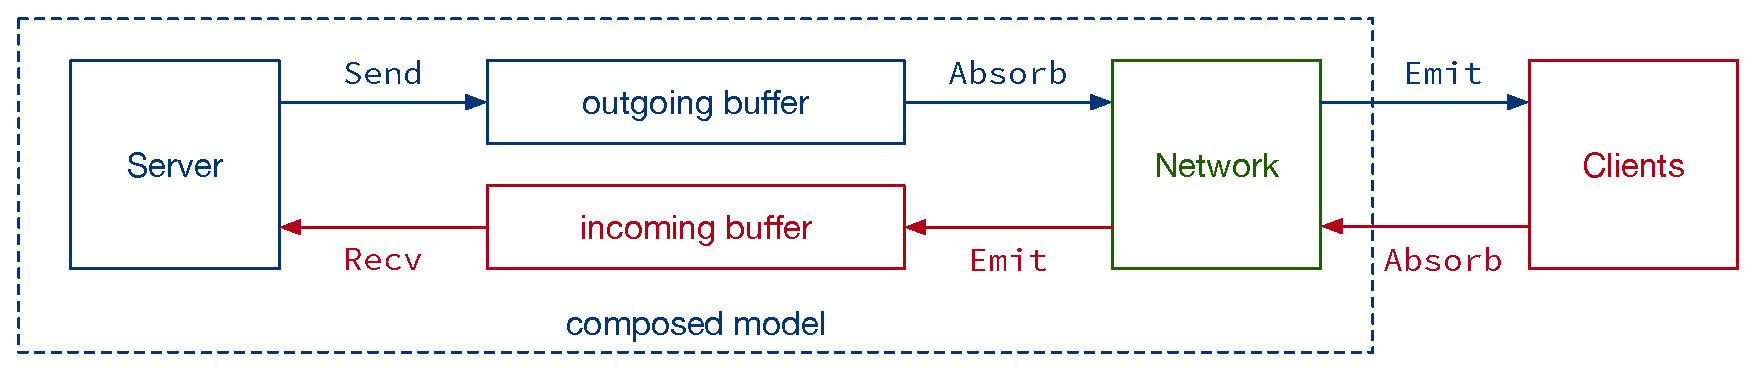
\includegraphics[width=\textwidth]{figures/net-compose}
  \caption{Network composition architecture}
  \label{fig:net-compose}
\end{figure}

To handle the asynchronicity among the server and network events, I insert
message buffers between them.  As shown in \autoref{fig:net-compose}, the {\em
  incoming buffer} stores the packets emitted by the network but not yet
consumed by the server's \ilc{Recv} events, and the {\em outgoing buffer} stores
the packets sent by the server but not yet absorbed by the network.

\begin{figure}
\begin{lstlisting}[style=customcoq,numbers=left,escapechar=\%]
CoFixpoint compose {E} (srv: itree (qaE +' E) void)   (* server  model *)
           (net  : itree (netE +' nondetE) void)      (* network model *)
           (bi bo: list packet)       (* incoming and outgoing buffers *)
           : itree (netE +' nondetE +' E) void :=
  let step_net :=%\label{line:step-net-def}%
    match net with
    | Impure (Absorb|) knet =>
      if bo is pkt::bo'
      then compose srv (knet pkt) bi bo'%\label{line:net-absorb}%
      else pkt <- trigger Absorb;;%\label{line:client-send}%
           compose srv (knet pkt) bi bo
    | Impure (Emit pkt|) knet =>
      if toServer pkt
      then compose srv (knet tt) (bi++[pkt]) bo%\label{line:srv-incoming}%
      else trigger (Emit pkt);;%\label{line:net-emit}%
           compose srv (knet tt) bi bo
    | Impure (|Or) knet => b <- trigger Or;;
                        compose srv (knet b) bi bo
    | Pure vd => match vd in void with end
    end
  in
  match srv with
  | Impure (Recv|) ksrv =>
    if bi is pkt::bi'
    then compose (ksrv pkt) net bi' bo%\label{line:srv-consume}%
    else step_net%\label{line:step-net}%
  | Impure (Send pkt|) ksrv =>%\label{line:srv-send}%
    compose (ksrv tt) net bi (bo++[pkt])
  | Impure (|e) ksrv =>        (* other events performed by the server *)
    r <- trigger e;; compose (ksrv r) net bi bo
  | Pure vd => match vd in void with end
  end.
\end{lstlisting}
\caption[Network composition algorithm]{Network composition algorithm.  When the
  server wants to send a packet in \autoref{line:srv-send}, the packet is
  appended to the outgoing buffer until absorbed by the network in
  \autoref{line:net-absorb}, and eventually emitted to the client in
  \autoref{line:net-emit}.  Conversely, packets sent by clients are absorbed by
  the network in \autoref{line:client-send}, emitted to the server's incoming
  buffer in \autoref{line:srv-incoming}, until the server consumes it in
  \autoref{line:srv-consume}.}
\label{fig:net-compose-code}
\end{figure}

The server and the clients are the opposite ends of the network.  Each packet
has routing fields that indicate its source and destination.  When the network
emits a packet, we need to determine whether the packet is emitted to the
server's incoming buffer or to the clients, by inspecting its destination:
\begin{coq}
  Record packet := {
    source      : connection;
    destination : connection;
    payload     : data
  }.

  Definition toServer (p: packet) : bool :=
    if p.(destination) is server_conn then true else false.
\end{coq}

Now we can define the composition algorithm formally, as shown in
\autoref{fig:net-compose-code}.  In this example, we reuse the \ilc{qaE}
definition in \autoref{sec:itree-lang}, and let the \ilc Q and \ilc A both be
the \ilc{packet} type.  The composed ITree takes the server and network models
as parameters, and makes steps in the two ITrees in certain order.

The composed model exhibits to the client three kinds of events: (i) Network
operations (\ilc{netE}) where packets are emitted to or absorbed from clients,
(ii) Nondetermistic branches (\ilc{nondetE}) made by the network model, and
(iii) Other events \ilc{\{E\}} performed by the server model {\it e.g.} internal
choices (\ilc{choiceE}) in \autoref{sec:itree-lang}.

Notice that this algorithm schedules the server at a higher priority than the
network model.  The composed model only steps into the network model when the
server is starved in \autoref{line:step-net}, by calling the \ilc{step_net}
process defined in \autoref{line:step-net-def}.  Such design is to avoid
divergence of the derived tester program, which I'll further explain in
\autoref{sec:backtrack}.

So far I've shown how to specify systems that exhibit external nondeterminism.
By specifying the environment and composing it with the implementation-side
specification, we can describe the space of valid observations.  The rest of
this chapter will show how to derive tester programs from the observer-side
specification.


\section{Handling Internal Nondeterminism}
\label{sec:internal-nondet}
This section applies the idea of dualization in \autoref{chap:dualize} to the
ITree context, showing how to address internal nondeterminism by symbolic
evaluation based on ITree specifications.  It covers the derivation path from
``symbolic model'' to ``nondeterministic tester'' in \autoref{fig:framework},
using \http entity tags introduced in \autoref{sec:internal-nondeterminism} as
an example.

As discussed in \autoref{sec:encode-spec}, dualization requires refining the
representation of the server's computation {\it e.g.} encoding its branches over
symbolic conditions.  This is done by designing ITrees' event types in
\autoref{sec:symbolic-model} and specifying the server's behavior with a
symbolic model.

The server specification is derived into a tester client by {\em interpreting}
interaction trees.  To interpret is to define semantic rules that transform one
ITree program into another, and corresponds to the arrows in
\autoref{fig:framework}.  \autoref{sec:interp} explains the interpretation of
ITrees.

The interpretation from symbolic model to the nondeterministic tester model is
implemented in two phases, illustrated as ``dualization'' and ``unification''
arrows in \autoref{fig:framework}: \autoref{sec:dualize-interaction} dualizes
the server's behavior into the tester client's, resulting in a ``symbolic
observer'' that encodes symbolic evaluation as primitive events.
\autoref{sec:symbolic-eval} then instantiates the primitive events into
pure computations that unify concrete observations against their symbolic
representations.

\subsection{Symbolic server model}
\label{sec:symbolic-model}
The server specification is an ITree program that exhibits all valid behavior of
the protocol.  I combine the $\Prog$ language in \autoref{sec:prog-lang} with the
simplistic ITree example in \autoref{sec:qac-itree}.

\paragraph{Network packet type}
Instead of receiving requests and sending responses, the server receives and
sends {\em packets} that carry routing information.  This allows us to specify
the server's interaction against concurrent clients in
\autoref{sec:external-nondet}.  A packet consists of headers that indicate its
source and destination, and a payload of either a request or a response:
\begin{coq}
  Notation connection := N. (* N for natural number *)

  Record packet Q A := {
    Source      : endpoint;
    Destination : endpoint;
    Payload     : Q + A
  }.
\end{coq}
This type definition says: the \ilc{packet} type is parameterized over the \ilc
Q and \ilc A types that represent its request and response.  Its \ilc{Source}
and \ilc{Destination} fields each records an \ilc{endpoint} represented as a
natural number.  Its \ilc{Payload} type is the sum of request and response.

Here's an example trace of network packets:
\begin{coq}
  Context get: string -> request.
  Context ok : string -> response.

  Definition server_end: endpoint := 0.

  Example trace: list (packet request response) :=
    [ { Source      := 1;
        Destination := server_end;
        Payload     := inl (get "/index.html")
      }
    ; { Source      := server_end;
        Destination := 1;
        Payload     := inr (ok "<p>Hello!</p>")
      }
    ].
\end{coq}
This trace encodes a transaction between client 1 and the server (represented as
endpoint 0).  The client sends a GET request to fetch the resource in path
\ilc{"/index.html"}, and the server responds with 200 OK and content
\ilc{"<p>Hello!</p>"}.  The \ilc{inl} and \ilc{inr} are constructors for sum
types:
\begin{coq}
  Context inl: forall {X Y}, X -> X + Y.
  Context inr: forall {X Y}, Y -> X + Y.
\end{coq}

\paragraph{Symbolic representation}
To specify systems' nondeterministic behavior, the $\Prog$ language in
\autoref{sec:prog-lang} encodes data as symbolic expressions $\Sexp$, so that
the responses and branch conditions may depend on internal choices.  I do the
same for ITree specifications, by symbolizing the choice events and branch
conditions.  Take my HTTP specification~\cite{issta21} as an example.  Its
choice event has symbolic expression as result type:

\begin{coq}
  Variant comparison := Strong | Weak.

  Variant exp: Type -> Type :=
    Const    : string -> exp string
  | Var      : var    -> exp string
  | Compare  : string -> exp string -> comparison -> exp bool.

  Variant choiceE: Type -> Type :=
    Choice: choiceE (exp string).
\end{coq}

Here I instantiate the \ilc{choiceE} in \autoref{sec:itree-lang} with symbolic
return type \ilc{(exp string)}, pronounced ``expression of type string''.  In
this example, I use strings to represent entity tags (ETags) that HTTP servers
may generate, which was discussed in \autoref{sec:internal-nondeterminism}.  The
type interface can be adjusted to other protocols under test.

Symbolic expressions may be constructed as constant values, as variables, or
with operators.  Here is an example of expressions of type string:
\begin{coq}
  Context x y : var.

  Example expressions: list (exp string) :=
    [ Const   "foo"
    ; Var      x
    ; Compare "bar" (Var y) Weak
    ].
\end{coq}

The \ilc{Compare} constructor takes an expression of type string and compares it
against a constant string.  \ilc{(Compare t tx cmp)} represents the ETag
comparison between \ilc{t} and \ilc{tx}, using ``strong comparison'' or ``weak
comparison'' mechanism\footnote{\http servers may choose to generate ETags as
``strong validators'' (with uniqueness guarantee) or ``weak validators'' (for
potentially better performance).  Weak validators have prefix \iletag{W/} while
strong validators do not.  When handling compare-and-swap operations such as PUT
requests conditioned over \inlinec{If-Match} in
\autoref{sec:internal-nondeterminism}, the server should evaluate its
precondition with ``strong comparison'' that doesn't allow weak validators ({\it
e.g.} \iletag{W/"foo"}) to match any ETag including itself.  For GET requests
conditioned over \inlinec{If-None-Match}, the server may evaluate with ``weak
comparison'' where a weak validator like \iletag{W/"bar"} matches itself and
also matches strong validator \iletag{"bar"}, but doesn't match \iletag{W/"foo"}
or \iletag{"foo"}.} specified by \ilc{cmp}.  The constant ETag is provided by
the request, and the symbolic one comes from the server state.

\begin{figure}
\begin{lstlisting}[numbers=left]
  Notation sigma := (path -> resource).

  Context OK PreconditionFailed : symbolic_response.
  Context process: request -> sigma -> itree smE (symbolic_response * sigma).

  CoFixpoint server_http (state: sigma) :=
    pq <- trigger Recv;;
    let respond_with a :=
      trigger (Send { Source      := server_conn
                    ; Destination := pq.(Source)
                    ; Payload     := inr a } ) in
    let q : request    := request_of pq        in
    let v : string     := q.(Content)          in
    let k : path       := q.(TargetPath)       in
    let t : string     := if_match q           in
    let tx: exp string := (state k).(ETag)     in
    IFX (Compare t tx Strong)%\label{line:etag-ifx}%
    THEN
      if q.(Method) is Put%\label{line:etag-pure-if}%
      then
        tx' <- or (trigger Choice)%\label{line:etag-choice}%
                  (Pure (Const EmptyString));;
        let state' := state [k |-> {Content := v; ETag := tx'}] in
        respond_with OK;;
        server_http state'
      else                 (* handling other kinds of requests *)
        (a, state') <- process q state;;
        respond_with a;;
        server_http state'
    ELSE
      respond_with PreconditionFailed;;
      server_http s.%\label{line:etag-end}%
\end{lstlisting}
\caption{Server model for HTTP conditional requests}
\label{fig:if-match-server}
\end{figure}

\autoref{fig:if-match-server} shows an ITree model for If-Match requests 
(\autoref{sec:internal-nondeterminism}).  The server state \ilc{sigma} \lys{I
used \ilc{sigma} to represent the server state in QAC, so keeping this
notation.}  maps each path to its corresponding ``resource''---file content and
metadata like ETag.  The server first evaluates the request's \inlinec{If-Match}
condition by ``strong comparison'' as required by HTTP.  If the request's ETag
matches its target's, then the server updates the target's contents with the
request payload.  The target's new ETag \ilc{tx'} is permitted to be any value,
so the model represents it as \ilc{Choice} event.

Notice that the server model exhibits three kinds of branches:
\begin{enumerate}
\item The \ilc{if} branch in \autoref{line:etag-pure-if} is provided by ITree's
embedding language Coq, and takes a boolean value as condition;
\item The \ilc{IFX} branch in \autoref{line:etag-ifx} constructs an ITree that
nondeterministically branches over a condition written as a symbolic expression
of type bool:
\begin{coq}
  Variant branchE: Type -> Type := (* symbolic-conditional branch *)
    Decide: exp bool -> branchE bool.

  Notation "IFX condition THEN x ELSE y" :=
    (b <- trigger (Decide condition);;
     if b then x else y).
\end{coq}
\item The \ilc{or} operator in \autoref{line:etag-choice} takes two ITrees
\ilc x and \ilc y as possible branches and constructs a nondeterministic program
that may behave as either \ilc x or \ilc y:
\begin{coq}
  Variant nondetE: Type -> Type := (* nondeterministic branch *)
    Or: nondetE bool.

  Definition or {E R} `{nondetE -< E} (x y: itree E R) : itree E R :=
    b <- trigger Or;;
    if b then x else y.
\end{coq}
Here \ilc{nondetE} is a special case of \ilc{choiceE} with boolean space of
choices, but they'll be handled differently during test derivation.  The type
signature \ilc{\{E R\} `\{nondetE -< E\}} says the \ilc{(or)} combinator can
apply to ITrees whose event \ilc E is a super-event of \ilc{nondetE}, and with
arbitrary return type \ilc R.  For example, arguments \ilc x and \ilc y can be
of type \ilc{(itree (qaE +' nondetE +' choiceE +' branchE) void)}.
\end{enumerate}

These three kinds of branch conditions play different roles in the
specification, and will be handled differently during testing:
\begin{enumerate}
\item The ``pure'' \ilc{if} condition is used for deterministic branches like
  \ilc{(q.(Method) is Put)} in the example.  Here \ilc q is a ``concrete
  request''---a request that doesn't involve symbolic variables, as opposed to
  ``symbolic'' ones---generated by the client and sent to the server, so its
  method is known by the tester and needn't be symbolically evaluated.
\item The ``symbolic'' \ilc{IFX} condition here plays a similar rule as the
  $\mathsf{if}$ branches in the $\Prog$ language: Which branch to take depends
  on the server's internal choices, so the tester needs to consider both cases.
\item The \ilc{or} branch defines multiple control flows the server may take.
  In the HTTP example, the server may generate an ETag for the resource's new
  content, but is not obliged to do so.  It may choose to generate no ETags
  instead, using \ilc{(Pure (Const EmptyString))} as an alternative
  to \ilc{(trigger Choice)}.
\end{enumerate}

In addition to \ilc{IFX} branch conditions, the symbolic expressions may also
appear in the server's responses.  For example, after generating an ETag in
\autoref{line:etag-choice} of \autoref{fig:if-match-server}, the server may
receive a GET request and send the ETag to the client:
\begin{coq}
  Example ok_with_etag: symbolic_response :=
    { ResponseLine := { Version := { Major := 1; Minor := 1 }
                      ; Code    := 200
                      ; Phrase  := OK
                      }
    ; ResponseFields :=
      [ { Name := "Content-Length"; Value := Const "13" }
      ; { Name := "ETag"          ; Value := Var    x   }
      ]
    ; ResponseBody := "<p>Hello!</p>"
    }.
\end{coq}
Suppose the server generated the ETag as expression \ilc{(Var x)}, then we can
use the expression to construct the symbolic response in the specification,
rather than determining its concrete value.  The mechanism of producing
expressions for ETags is explained in \autoref{sec:dualize-interaction}.

Now we can define the specification's event type \ilc{smE}.  The symbolic server
model receives concrete requests and sends symbolic responses, so its event is
defined as:
\begin{coq}
  Definition symbolic_packet := packet request symbolic_response.%\label{def:symbolic-packet}%

  Definition qaE := ioE symbolic_packet symbolic_packet.%\label{def:symbolic-qae}%

  Notation smE := (qaE +' nondetE +' choiceE +' branchE).
\end{coq}
The ``Symbolic Model'' in \autoref{fig:framework} is an ITree constructed by
applying the \ilc{server_http} function to an initial state:
\begin{coq}
  Definition sm_http: itree smE void :=
    server_http init_state.
\end{coq}

The rest of this section will explain the interpretations from this symbolic
model.

\subsection{Dualizing symbolic model}
\label{sec:dualize-interaction}
This subsection takes the symbolic model composed in
\autoref{sec:symbolic-model} and dualizes its interactions, which corresponds
to the ``Dualization'' arrow in \autoref{fig:framework}.  It applies the idea of
derivation rules (\ref{rule:write})--(\ref{rule:return}) for $\Prog$
(\autoref{sec:dualize-prog}) to models written as ITrees.

This interpretation phase produces a symbolic observer that models the tester's
observation and validation behavior.  The observer sends a request when the
server wants to receive one, and receives a response when the server wants to
send one.  It also creates constraints over the server's internal choices based
on its observations.

\autoref{fig:symbolic-observer} shows the dualization algorithm.  It interprets
the symbolic model's events with the \ilc{observe} handler, whose types are
explained as follows:

\begin{figure}
\begin{lstlisting}[numbers=left]
Notation oE := (observeE +' nondetE +' choiceE +' constraintE).

Definition observe {R} (e: smE R) : itree oE R :=
  match e with
  | Recv      => trigger FromObserver%\label{line:observe-absorb}%
  | Send px   => p <- trigger ToObserver;;%\label{line:observe-emit}%
                 trigger (Guard px p)
  | Decide bx => or (trigger (Unify bx true);;  ret true)%\label{line:observe-branch}%
                    (trigger (Unify bx false);; ret false)
  | Or        => trigger Or%\label{line:observe-or}%
  | Choice    => trigger Choice%\label{line:observe-choice}%
  end.

Definition observer_http: itree oE void :=
  interp observe sm_http.
\end{lstlisting}
\caption{Dualizing symbolic model into symbolic observer.}
\label{fig:symbolic-observer}
\end{figure}

The tester observes a trace of concrete packets, so observer's interactions
return concrete requests and responses, as opposed to the symbolic model whose
responses are symbolic.
\begin{coq}
  Definition concrete_packet := packet request concrete_response.

  Variant observeE : Type -> Type :=
    FromObserver   : observeE concrete_packet
  | ToObserver     : observeE concrete_packet.
\end{coq}

Notice that the observer's send and receive events both return the packet sent
or received, unlike the server model whose \ilc{Send} event takes the sent
packet as argument.  This is because the tester needs to generate the request
packet to send, and the event's result value represents that generated and sent
packet.

As discussed in \autoref{sec:dualize-prog}, when the server sends a symbolic
response or branches over a symbolic condition, the tester needs to create
symbolic constraints accordingly.  The observer introduces ``constraint events''
to represent the creation of constraints primitively.
\begin{coq}
  Variant constraintE : Type -> Type :=
    Guard : packet -> concrete_packet -> constraintE unit
  | Unify : exp bool -> bool -> constraintE unit.
\end{coq}

Here \ilc{(Guard px p)} creates a constraint that the symbolic packet \ilc{px}
emitted by the specification matches the concrete packet \ilc p observed during
runtime.  \ilc{(Unify bx b)} creates a constraint that unifies the symbolic
branch condition \ilc{bx} with boolean value \ilc b.  These constraints will be
solved in \autoref{sec:symbolic-eval}.

The dualization algorithm in \autoref{fig:symbolic-observer} does the follows:
\begin{enumerate}
  \item When the symbolic model absorbs a packet in
    \autoref{line:observe-absorb}, the observer generates a request packet;
  \item When the symbolic model emits a symbolic packet \ilc{px} in
    \autoref{line:observe-emit}, the observer receives a concrete packet \ilc p,
    and adds a constraint that restricts the symbolic and concrete packets to
    match each other.
  \item When the symbolic model branches on a symbolic condition \ilc{bx} in
    \autoref{line:observe-branch}, the tester accepts the observation if it can
    be explained by any branch.  This is done by constructing the observer as a
    nondeterministic program that has both branches, using the \ilc{or}
    combinator.  For each branch, the observer adds a constraint that the
    symbolic condition matches the chosen branch.
  \item Nondeterministic branches in \autoref{line:observe-or} are preserved in
    this interpretation phase, and will be resolved in \autoref{sec:backtrack}.
  \item Internal choices in \autoref{line:observe-choice} are addressed by the
    next phase in \autoref{sec:symbolic-eval}, along with the constraints
    created in this phase.
\end{enumerate}

The result of dualization is a symbolic observer that models tester behaviors
like sending requests and receiving responses.  The symbolic observer is a
nondeterministic program with primitives events like making choices and adding
constraints over the choices.

For example, dualizing \autoref{line:etag-ifx}--\ref{line:etag-end} in
\autoref{fig:if-match-server} results in an observer program as shown in
\autoref{fig:observer-example}.  The next subsection interprets the observer's
primitive \ilc{Guard} and \ilc{Unify} events into pure computations of symbolic
evaluation.

\begin{figure}
\begin{coq}
  Example observer_body: itree oE void :=
    let guard_response a :=
      p <- trigger ToObserver;;
      trigger (Guard { Source      := server_conn
                     ; Destination := pq.(Source)
                     ; Payload     := inr a } ) in
    let bx: exp bool := Compare t tx Strong in
    or (
        trigger (Unify (Compare bx true));;
        if q.(Method) is Put
        then
          tx' <- or (trigger Choice)
                    (Pure (Const EmptyString));;
          let state' := state [k |-> {Content := v; ETag := tx'}] in
          guard_response OK;;
          interp observe (server_http state')
        else
          (a, state') <- interp observe (process q state);;
          guard_response a;;
          interp observe (server_http state')
       )
       (
        trigger (Unify (Compare bx false));;
        guard_response PreconditionFailed;;
        interp observe (server_http s)
       ).
\end{coq}
\caption{Symbolic observer example.}
\label{fig:observer-example}
\end{figure}


\subsection{Symbolic evaluation}
\label{sec:symbolic-eval}
This subsection takes the symbolic observer produced in
\autoref{sec:dualize-interaction} and solves the constraints it has created.
The constraints unify symbolic packets and branch conditions against the
concrete observations.  The tester should accept the SUT if the constraints are
satisfiable.

\begin{figure}
\begin{lstlisting}[numbers=left]
Notation ntE := (observeE +' nondetE +' exceptE).

Definition V: Type := list var * list (constraintE unit).
  
Definition unify {R} (e: oE R) (v: V) : itree ntE (V * R) :=
  let (xs, cs) := v in
  match e with
  | Choice => let x: var := fresh v in%\label{line:unify-choice}%
              ret (x::xs, cs, Var x)
  | (constraint: unifyE) => let cs' := constraint::cs in%\label{line:unify-constraint}%
                            if solvable cs'
                            then ret (xs, cs', tt)
                            else Trigger (Throw ("Conflict: " ++ print cs'))
  | Or             => b <- trigger Or;; ret (v, b)%\label{line:unify-or}%
  | (oe: observeE) => r <- trigger oe;; ret (v, r)%\label{line:unify-observe}%
  end.

Definition nondet_tester_http: itree ntE void :=
  (_, vd) <- interp_state unify observer_http initV;;
  match vd in void with end.
\end{lstlisting}
\caption{Resolving symbolic constraints.}
\label{fig:nondet-tester}
\end{figure}

As shown in \autoref{fig:nondet-tester}, the unification algorithm evaluates the
primitive symbolic events into a stateful checker program, which reflects the
$\Prog$-based validator in \autoref{sec:dualize-prog}.  The interpreter
maintains a validation state \ilc V which stores the symbolic variables and the
constraints over them.  The derivation rules are as follows:
\begin{enumerate}
  \item When the server makes an internal choice in \autoref{line:unify-choice},
    the tester creates a fresh variable and adds it to the validation state.
  \item When the observer creates a constraint in
    \autoref{line:unify-constraint}, the tester adds the constraint to the
    validation state, and solves the new set of constraints.  If the constraints
    become unsatisfiable, then the tester \ilc{Throw}s an exception that
    indicates the current execution branch cannot accept the observations:
\begin{coq}
  Variable exceptE: Type -> Type :=
    Throw: forall {X}, string -> exceptE X.
\end{coq}
  \item The observer is a nondeterministic program with multiple execution
    paths, constructed by \ilc{Or} events in \autoref{line:unify-or}.  The
    tester accepts the observation if any of the branches does not throw an
    exception.  These branches will be handled in the next section, along with
    the observer's send/receive interactions in \autoref{line:unify-observe}.
\end{enumerate}

Notice that the \ilc{unify} function interprets a symbolic observer's event
\ilc{(oE R)} into a function of type \ilc{(V -> itree tE (V * R))},
called ``state monad transformer''.  It takes a pre-validation state \ilc{(v:
V)} and computes an ITree that yields the observer event's corresponding result
\ilc{(r: R)} along with a post-validation state \ilc{(v': V)}.  This stateful
interpretation process is implemented by a variant of \ilc{interp} called
\ilc{interp_state}:
\begin{coq}
  CoFixpoint interp_state {E F V R}
                          (handler: forall {X}, E X -> V -> itree F (V * X))
                          (m: itree E R) (v: V)
             : itree F (V * R) :=
    match m with
    | Pure   r   => ret (v, r)
    | Impure e k => '(v', r) <- handler e v;;
                    interp_state handler (k r) v'
    end.
\end{coq}

So far I have interpreted the symbolic model into a tester model that observes
incoming and outgoing packets, nondeterministically branches, and in some cases
throws exceptions.  In this section, I used the server model verbatim as the
symbolic model, and the derived tester can handle internal nondeterminism by
symbolic evaluation.

The server model's receive and send events are linear.  It doesn't receive new
requests before responding to its previous request.  As a result, the tester
dualized from the server model doesn't send new requests before it receives the
response to the previous request, so it doesn't reveal the server's interaction
with multiple clients simultaneously.  In the next section, I'll explain how to
create a multi-client tester by extending the symbolic model, addressing
external nondeterminism.


\section{Executing Tester Model}
\label{sec:backtrack}

This section shows how to derive the specification into an interactive tester
program, using networked servers as an example.  I take the dualization theory
in \autoref{chap:theory} and apply it to the ITree specification language.

  The network composition phase was
explained in \autoref{sec:net-compose}, and this section describes the remainder
of the framework.

\subsection{Dualizing ITree model}
\label{sec:symbolic-observer}
To {\em observe} the server's behavior, we have to interpret the specified
server-side events into tester-side events: When the server should send a
certain message, the tester expects to receive the specified message, and
rejects the server upon receiving an unexpected message; when the server should
receive some message, the tester generates a message and sends it to the server,
as shown in \autoref{fig:sym-observe}.

\begin{figure}
  \begin{coq}
let observe (server) =
  match server with
  | pkt := recv(); s'(pkt) =>
    p := gen_pkt(); send(p); observe (s'(p))
  | send(pkt); s' =>
    p := recv(); guard(pkt, p); observe (s')
  | IF (x, s1, s2) =>
    (* Allow validating observation with [s1],
     * provided [x] is unifiable with [true];
     * Or, unify [x] with [false],
     * and validate observation with [s2]. *)
    determine(unify(x, true ); observe (s1),
              unify(x, false); observe (s2))
  | r  := _(); s'(r) =>
    r1 := _(); observe (s'(r1))
  end
  \end{coq}
  \caption{Dualizing server model into observer model.  Upon \ilc{recv} events,
    the observer generates a packet and sends it to the server.  For \ilc{send}
    events, the observer receives a packet \ilc{p1}, and fails if it does not
    match the specified \ilc{pkt}.  When the server makes nondeterminstic
    \ilc{IF} branches, the observer \ilc{determine}s between the branches by
    \ilc{unify}ing the branch condition with its conjectured value, and then
    observing the corresponding branch.
    %% Such unification may fail immediately, or add a constraint to the
    %% symbolic variables in \ilc{x}, which instructs future
    %% observations. \bcp{??}
  }
  \label{fig:sym-observe}
\end{figure}

Besides sending and receiving messages, the model also has \ilc{IF} branches
conditioned over symbolic expressions, like that shown in
\autoref{fig:if-match-model}.  Upon nondeterministic branching, the tester needs to
determine which branch was actually taken, by constructing observers for both
branches.  Each branch represents a possible explanation of the server's
behavior.  Upon further interacting with the server, some branches might fail
because its conjecture cannot explain what it has observed.  The tester rejects
the server if all branches have failed, indicating that the server corresponds
to no possible case in the model.
%% \bcp{Very confusing.}

Dualizing the server-side model produces an observer model that performs
interactions to reveal the server's behavior and check its validity.  This model
includes all possible observations from a valid server, and needs to
\ilc{determine} which branch in the server model matches the observed behavior.
The model validates its observations with unification events \ilc{unify} and
\ilc{guard}.  These primitive events are handled by later interpretations: The
\ilc{unify} and \ilc{guard} events in each branch are instantiated into symbolic
evaluation logic that decides whether this branch should fail or not; The
\ilc{determine} events are instantiated into backtracking searches to find if
all branches have failed, which rejects the server.


\subsection{Symbolic Evaluation}
\label{sec:symbolic-evaluation}
\begin{figure}
  \begin{lstlisting}[style=customcoq,numbers=left,escapechar=\%]
(* unifyS = list variable * list constraint    *)
(* new_var : unifyS -> variable * unifyS        *)
(* assert : exp T * T * unifyS -> option unifyS *)
let unifier (observer, map : mcid -> pcid,
         vars : unifyS) =
  match observer with
  | x := fresh(); o'(x) =>
    let (x1, vars') = new_var(vars) in
    unifier (o'(x1), vars', map)
  | unify(x, v); o' =>
    match assert(x, v, vars) with
    | Some vars' => unifier (o', vars', map)
    | None => failwith "Unexpected payload"
    end
  | guard(p0, p1); o' =>
    match assert(p0, p1, vars) with
    | Some vars' => unifier (o', vars', map)
    | None => failwith "Unexpected payload"
    end
  | r  := _(); o'(r) =>
    r1 := _(); unifier (o'(r1), vars, map)
  end\end{lstlisting}
  \caption{Instantiating symbolic events.  The tester maintains a \ilc{unifyS}tate
    which stores the constraints on symbolic variables.  When the
    specification creates a \ilc{fresh} symbol, the tester creates an entry for
    the symbol with no initial constraints.  Upon \ilc{unify} and
    \ilc{guard} events, the tester checks whether the \ilc{assert}ion is
    compatible with the current constraints.  If yes, it updates the constraints
    and move on; otherwise, it raises an error on the current branch.
    %% \sz{We should mention the \ilc{fresh} operation in the main text!}
  }
  \label{fig:unifier}
\end{figure}

In this interpretation phase, we handle nondeterminism at data level by handling
\ilc{fresh} events in the server model, as well as \ilc{unify} and \ilc{guard}
events introduced by dualization.  The interpretor instantiates these events
into symbolic evaluation algorithms.

As shown in \autoref{fig:unifier}, the tester checks whether the observed/conjectured
value matches the specification, by maintaining the constraints on the symbolic
variables.  These constraints are initially empty when the variables are
generated by \ilc{fresh} events.  As the test runs into \ilc{unify} and
\ilc{guard} events, it adds constraints \ilc{assert}ing that the observed value
matches the specification, and checks whether the constraints are still
compatible.  Incompatibility among constraints indicates that the server has
exhibited behavior that cannot be explained by the model, implying violation
against the current branch of specification.

\subsection{Backtracking}
\label{sec:backtracking}
\begin{figure}
  \begin{coq}[escapechar=\%]
(* filter : event T * T * list M -> list M *)
(* [filter(e, r, l)] returns a subset in [l],
 * where the model programs' next event is [e]
 * that returns [r]. *)
let backtrack (current, others) =
  match current with
  | determine(t1, t2) =>
    backtrack (t1, t2::others)
  | failwith error => (* current branch failed *) %\label{line:begin-failure}%
    match others with
    | [] => failwith error
    | another::ot' => backtrack (another, ot')
    end %\label{line:end-failure}%
  | send(pkt); t' =>
    let ot' = filter(SEND, pkt, others) in %\label{line:filter-send}%
    send(pkt); backtrack (t', ot')
  | pkt := recv(); t'(pkt) =>
    opkt := maybe_recv();
    match opkt with
    | Some p1 =>
      let ot' = filter(RECV, pkt, others) in %\label{line:filter-recv}%
      backtrack (t'(p1), ot')
    | None =>             (* no packet arrived *)
      match others with
      | [] => backtrack (current, []) (* retry *)
      | another::ot' =>            (* postpone *)
        backtrack (another, ot'++[current])
      end
    end
  end in
backtrack (tester_nondet, [])
  \end{coq}
  \caption{From nondeterministic model to deterministic tester program.  If the
    model makes nondeterministic branches, the tester picks a branch to start
    with, and puts the other branch into a set of other possibilities.  If the
    current branch has failed, the tester looks for other possible branches to
    continue checking.  When the current branch sends a packet, the tester
    filters the set of other possibilities, and only keeps the branches that
    match the current send event.  If the model wants to receive a packet, the
    tester handles both cases whether some packet has arrived or not.}
  \label{fig:backtrack}
\end{figure}

Symbolic evaluation determines whether the observations matches the tester's
conjectures on each branch.  So far, the derived tester
is a nondeterministic program that rejects the server if and only if all
possible branches have raised some error.  To simulate this tester on a
deterministic machine, we execute one branch until it fails.  Upon failure in
the current branch, the simulator switches to another possible branch, until it
exhausts all possibilities and rejects the server, as shown in
\autoref{line:begin-failure}--\ref{line:end-failure} of
\autoref{fig:backtrack}.

When switching from one branch to another, the tester cannot revert its previous
interactions with the server.  Therefore, it must match the server model against
all interactions it has performed, and filter out the mismatching branches, as
shown in \autoref{line:filter-send} and \autoref{line:filter-recv} of
\autoref{fig:backtrack}.
%% , utilizing the lazy evaluation nature of our
%% specification language.\sz{Mention this earlier when introducing Galina?}

We've now derived a tester from the server model.  The specified server runs
forever, and so does the tester (upon no violations observed).  We accept the
server if the tester hasn't rejected it after some large, pre-determined number
of steps of execution.


\chapter{Test Harness Design}
\label{chap:harness}
A tester consists of a validator and a test harness.  Chapters~\ref{chap:theory}
and \ref{chap:practices} have explained the validator's theory and practices.
This chapter presents a language-based design for test harnesses.  I'll show how
to generate and shrink test inputs effectively, addressing inter-execution
nondeterminism.

\autoref{sec:harness-overview} provides a brief overview of how test harnesses
work.  \autoref{sec:heuristics} explains how to write heuristics to generate
interesting test inputs.  \autoref{sec:shrinking} then shows how to keep the
test inputs interesting among different executions in the shrinking process.

\section{Overview}
\label{sec:harness-overview}
\begin{figure}
  \centering
  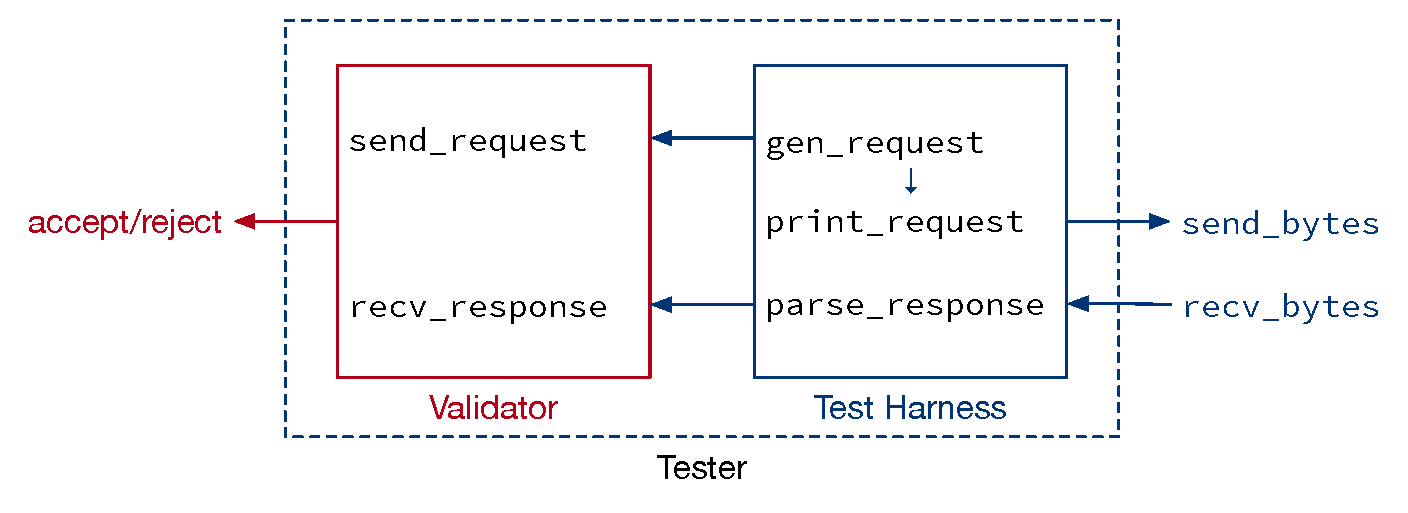
\includegraphics[width=.9\textwidth]{figures/harness-outline}
  \caption{Tester architecture outline.}
  \label{fig:overview}
\end{figure}

This section introduces the abstract architecture of an interactive tester,
using the networked server as an example.  I'll present a na\"ive implementation
of the test harness, which will be improved in the following sections.

The test harness interacts with the environment and provides the observations
for the validator.  The validator may represent requests and responses as
abstract datatypes for the convenience of specification.  The test harness
translates these abstract representations into bytes transmitted on the
underlying channel.

As shown in \autoref{fig:overview}, when the validator wants to observe a sent
request, the harness generates the request and encodes it into bytes to send.
Conversely, when the validator wants to observe a received response, the harness
receives bytes from the environment and decodes them into abstract messages.

\begin{figure}
\begin{lstlisting}[numbers=left]
Definition gen_packet: IO concrete_packet :=
  src          <- random_conn;;
  method       <- oneof [Get; Put];;
  target       <- random_path;;%\label{line:random-path}%
  precondition <- oneof [IfMatch, IfNoneMatch];;
  etag         <- random_etag;;
  payload      <- random_string;;
  ret { Source      := src;
        Destination := server_conn;
        Data        := inr { Method     := method;
                             TargetPath := target;
                             Headers    := [(precondition, etag)];
                             Payload    := payload
                           }
      }.
\end{lstlisting}
\caption{Na\"ive generator for HTTP requests.}
\label{fig:naive-generator}
\end{figure}

A generator is a randomized program that produces test inputs.  One example is
the \ilc{gen_packet} function in \autoref{fig:execute}.  The HTTP packet
generator can be na\"ively implementation as shown in
\autoref{fig:naive-generator}.  It fills in the request's fields with arbitrary
values, and has limited coverage of the SUT's behavior.  This is because the
request target and ETags are both generated randomly, but a request is
interesting only if its ETag matches its target's corresponding resource stored
on the server.  A randomly generated request would result in 404 Not Found and
412 Precondition Failed in almost all cases.

To reveal more interesting behavior from the SUT, we should tune the generator's
distribution to emphasize certain patterns of the test input.  For example, if
the tester knows the set of paths where the server has stored resources, then it
can generate more paths that correspond to existing resources; if the tester has
observed some ETags generated by the server, then it can include these ETags in
future requests.  In the next section, I'll explain how to implement such
heuristics in ITree-based testers.


\section{Heuristics for Test Generation}
\label{sec:heuristics}
This section implements heuristics for generating test inputs.  I'll use the
HTTP tester as an example to show how to make requests more interesting by
parameterizing them over the model state (\autoref{sec:heuristic-state}) and the
trace (\autoref{sec:heuristic-trace}).

\subsection{State-based heuristics}
\label{sec:heuristic-state}
\paragraph{Motivation}
The model state may instruct the test generator to produce more interesting test
inputs.  For example, consider the \ilc{random_path} generator in
\autoref{line:random-path} of \autoref{fig:naive-generator}.  One way to improve
it is to generate more paths that have corresponding resources on the server:
\begin{coq}
  Definition gen_path (state: list (path * resource)) : IO path :=
    let paths: list path := map fst state in
    freq [(90, oneof paths);
          (10, random_path)].
\end{coq}

Here I modify the server model's state type \ilc{sigma} from \ilc{(path ->
  resource)} in \autoref{fig:if-match-server} into \ilc{(list (path *
  resource))}, which allows the generator to access the list of all \ilc{paths}
  in the server state.  The generator chooses from these existing paths in 90\%
  of the cases, as assigned by the \ilc{freq} combinator.  The remaining 10\%
  are still generated randomly, to discover how the SUT handles nonexistent
  paths.

For the \ilc{gen_packet} generator in \autoref{fig:naive-generator}, replacing
its \ilc{random_path} with the improved \ilc{gen_path} would generate more
interesting request targets.  This requires the \ilc{gen_packet} function to
carry the server state to instantiate \ilc{gen_path}.

As shown in \autoref{fig:backtrack}, the \ilc{GenPacket} generator is triggered
when the tester wants to observe a packet from itself to the SUT.
\autoref{fig:symbolic-observer} then shows that such \ilc{FromObserver} expectation
happens when the symbolic model \ilc{Send}s a packet.  Such a \ilc{Send} event
only happens when the server wants to receive a packet in
\autoref{fig:net-compose}.  The \ilc{Recv} events are triggered by the server
model in \autoref{fig:if-match-server}, which iterates over the server state
\ilc{sigma}.

\paragraph{Implementation}
To expose the server state to the request generator, I extend the symbolic
server model's \ilc{Recv} event type on Page~\pageref{def:symbolic-qae} to
include the server state:
\begin{coq}
  Variant qaE: Type -> Type :=
    Recv : sigma      -> qaE packet
  | Send : packet -> qaE unit.
\end{coq}

Now when the server wants to receive a request, it triggers \ilc{(Recv state)},
where \ilc{(state: sigma)} contains the server's paths and resources at that
point.  The \ilc{state} argument is then carried to the generator, by adding
parameters to the event types along the interpretation:
\begin{coq}
  Variant netE: Type -> Type :=
    Emit  : packet -> netE unit
  | Absorb: sigma      -> netE packet.

  Variant observeE : Type -> Type :=
    FromObserver   : sigma -> observeE concrete_packet
  | ToObserver     : observeE concrete_packet.

  Variant genE: Type -> Type :=
    GenPacket : sigma -> genE concrete_packet
  | GenBool   : genE bool.

  Definition gen_packet: sigma -> IO concrete_packet.
\end{coq}

\begin{figure}
\includegraphics[width=.6\linewidth]{figures/stategen}
\caption{State-based heuristics.}
\label{fig:stategen}
\end{figure}

As a result, when instantiating the \ilc{(GenPacket state)} event in
\autoref{fig:execute}, we can feed the \ilc{gen_packet} function with argument
\ilc{state}, so that \ilc{gen_path} can generate interesting paths based on the
server state.  \autoref{fig:stategen} illustrates this state-based heuristics.
It refines the test harness box in \autoref{fig:overview}, and will be extended
with trace-based heuristics in the next subsection.

\subsection{Trace-based heuristics}
\label{sec:heuristic-trace}

When the SUT makes internal choices, \eg, generating ETags, the
specification represents them as symbolic variables.  These variables' concrete
value are not stored in the specification state, but may be observed during
execution.  For example, when an HTTP server responds to a GET request, it might
include the resource's ETag as shown in \autoref{sec:internal-nondeterminism}.

To improve the generator in \autoref{fig:naive-generator}, we can generate
interesting ETags based on the trace produced during execution.  The trace is a
list of packets sent and received by the tester, and the packets' payloads may
include responses that have an ETag field.  The \ilc{gen_etag} function
emphasizes ETags that were observed in the trace, which are more likely to match
those generated by the SUT:
\begin{coq}
  Definition gen_etag (trace: list concrete_packet) : IO string :=
    let etags: list string := tags_of trace in
    freq [(90, oneof etags);
          (10, random_etag)].
\end{coq}

To utilize this improved generator for ETags, the tester needs to record the
trace of packets sent and received.  This is done by modifying the \ilc{execute}
function in \autoref{fig:execute}, adding an accumulator called ``\ilc{trace}''
as the recursion parameter:
\begin{coq}
  Fixpoint execute (fuel: nat) (trace: list concrete_packet)
                   (m: itree tE void) : IO bool :=
    match fuel with
    | S fuel' =>
      match m with
      | Impure e k =>
        match e with
        | (ClientSend q|) => client_send q;;
                             execute fuel' (trace ++ [q]) (k tt)
        | (ClientRecv|)   => oa <- client_recv;;                             
                             let trace' := match oa with
                                           | Some a => trace ++ [a]
                                           | None   => trace
                                           end in
                             execute fuel' trace' (k oa)
        | (|GenPacket state|) => pkt <- gen_packet state trace;;
                                 execute fuel' trace (k pkt)
        ... (* similar to %\autoref{fig:execute}% *)
\end{coq}
\lys{\ilc{trace ++ [q]} is indeed less inefficient than storing a reversed trace,
but this code is to show the concept of ``appending'' requests and responses to
a trace, and assumes that readers have the ability of optimizing its
performance.}

When the tester sends or receives a packet, the packet is appended to the
runtime \ilc{trace}.  Then the \ilc{gen_packet} generator can take the trace
accumulated so far and feed it to the ETag generator:
\begin{coq}
  Definition gen_packet (state: sigma) (trace: list concrete_packet) :=
    target <- gen_path state;;
    etag   <- gen_etag trace;;
    ... (* same as %\autoref{fig:naive-generator}% *)
\end{coq}

\begin{figure}
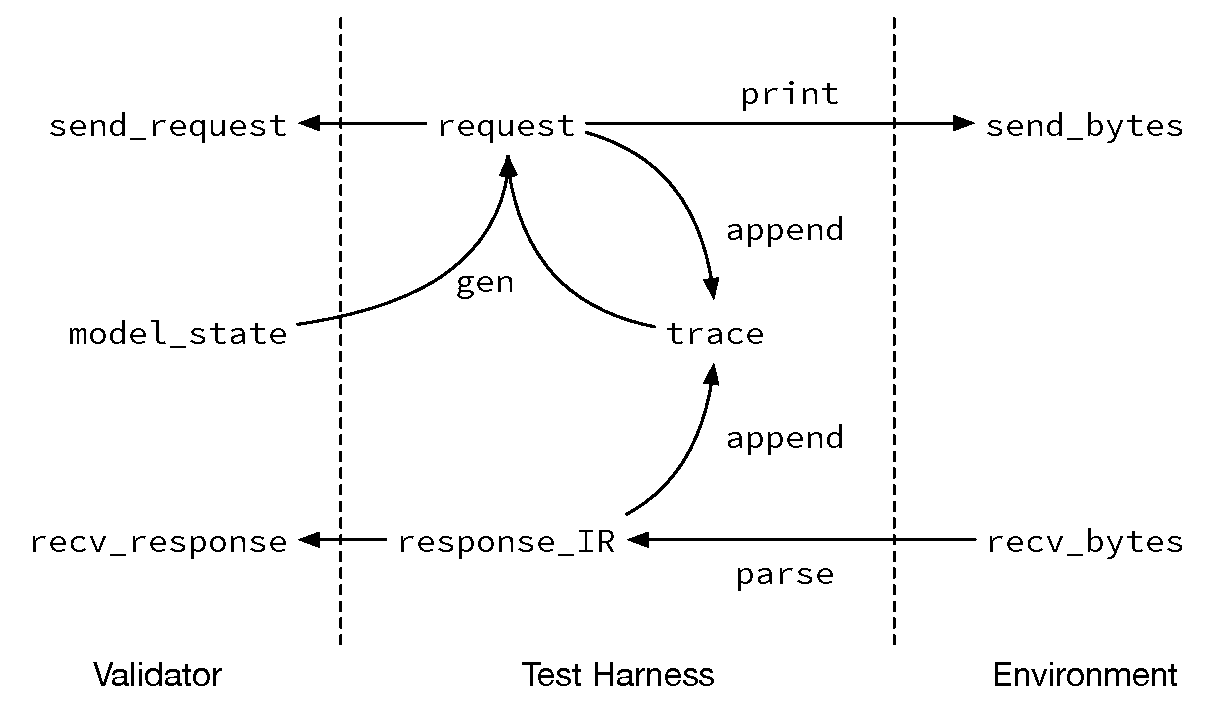
\includegraphics[width=.7\linewidth]{figures/gen}
\caption{Combining state-based and trace-based heuristics.}
\label{fig:gen}
\end{figure}

Now we can generate interesting test inputs by combining state-based and
trace-based heuristics, as shown in \autoref{fig:gen}.  In the next section,
I'll further extend this framework and shrink the test inputs while keeping them
interesting, addressing inter-execution nondeterminism.


\section{Shrinking Interactive Tests}
\label{sec:shrinking}
Suppose we have generated a test input that has caused invalid observations of
the SUT.  The generated counterexample consists of (1) {\em signal} that is
essential to triggering violations, and (2) {\em noise} that does not contribute
to revealing such violations.  We need to shrink the counterexample by removing
the noise and keeping the signal.

For interactive testing, the test input is a sequence of request messages.  An
intuitive way of shrinking is to remove some requests from the original sequence
and rerun the test.  However, rerunning an interesting request might produce
trivial results, due to inter-execution nondeterminism discussed in
\autoref{sec:inter-execution}.

To prevent turning signal into noise when rerunning the test, I shrink the
heurestics instead of shrinking the generated test input.
\autoref{sec:shrink-architecture} introduces the architecture for interactive
shrinking, then \autoref{sec:shrink-ir} explains the language design beneath
that addresses inter-execution nondeterminism.

\subsection{Architecture}
\label{sec:shrink-architecture}

I propose a generic framework for generating and shrinking interactive tests.
The key idea is to introduce an abstract representation for test inputs that
embeds trace-based heuristics.  When shrinking the counterexample, the test
harness picks a substructure of the abstract representation, and computes the
corresponding test input using the new runtime trace.

For example, when generating a timestamp, instead of producing concrete value,
e.g., ``\httpdate\today~\currenttime~GMT'', the generator returns an abstract
representation that says ``use the timestamp observed in the last response''.
When rerunning the test, the timestamp is computed from the new trace, e.g.,
``\httpdate\DayAfter~\currenttime~GMT''.

\begin{figure}
  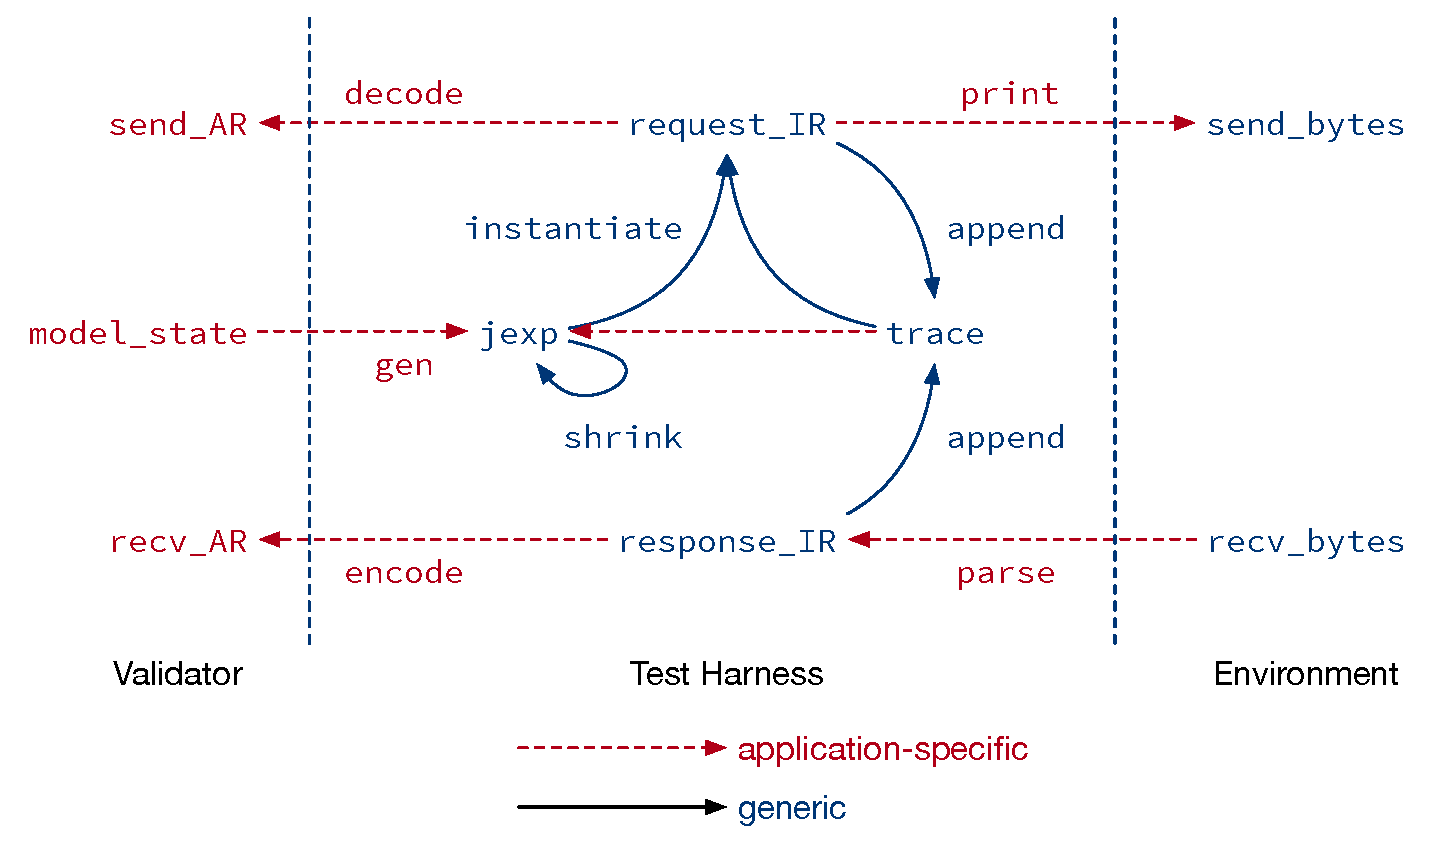
\includegraphics[width=.8\textwidth]{figures/shrink}
  \caption{Complete architecture of the test harness.}
  \label{fig:shrink}
\end{figure}

The test generation and shrinking framework is shown in \autoref{fig:shrink}.
It involves four languages, from right to left:
\begin{enumerate}
  \item Byte representation, in which the tester interacts with the environment.
    This can be network packets, file contents, or other serialized data
    produced and observed by the tester.
  \item Intermediate representation (IR), a generic language that abstracts the
    byte representation as structured data.  The test harness {\em parses} byte
    observations and records its trace in terms of the IR, which allows
    representing trace-based heuristics as a generic language, i.e.,
    J-expressions.
  \item J-expression (Jexp), a symbolic abstraction of the IR.  The IR
    corresponds to concrete inputs and outputs, whereas Jexp defines a
    computation from trace to IR.  The generator provides test inputs in terms
    of Jexps; The test harness {\em instantiates} the generated Jexps into
    request IR, and {\em prints} them into byte representation.

    When shrinking test inputs, the test harness shrinks the sequence of Jexps.
    The shrunk Jexps are then instantiated by the new trace during runtime.

    The intermediate representation and J-expression will be further explained
    in \autoref{sec:shrink-ir}.
  \item Application representation (AR), including the request (\ilc Q),
    response (\ilc A), and state (\ilc S) types used for specifying the
    protocol.  Specification writers can choose the type interface at their
    convenience, provided the request and response types are embeddable into the
    IR.
\end{enumerate}

The testing framework implements protocol-independent mechanisms like recording
the trace and shrinking counterexamples, which correspond to the blue solid
arrows in \autoref{fig:shrink}.  It can be used for testing various protocols,
provided application-specific translations from IR to AR and between IR and
bytes, illustrated as red dotted arrows.  The test developer needs to tune the
generator that produces Jexps, encoding their domain knowledge as state-based
and trace-based heuristics.

\subsection{Abstract representation languages}
\label{sec:shrink-ir}
I choose JSON as the IR in this framework, which allows syntax trees to be
arbitrarily wide and deep, and provides sufficient expressiveness for encoding
message data types in general.

\begin{figure}
\[\begin{array}{r@{\;}l}
\mathsf{JSON^T}\triangleq&\mathsf T\mid\{\mathsf{object^T}\}\mid[\mathsf{array^T}]\mid\mathsf{string}\mid\Int\mid\Bool\mid\mathsf{null}\\
\mathsf{object^T}\triangleq&\nil\mid\mathsf{"string": JSON^T,object^T}\\
\mathsf{array^T}\triangleq&\nil\mid\mathsf{JSON^T,array^T}\\
\mathsf{IR}\triangleq&\mathsf{JSON^{IR}}\\
\mathsf{Jexp}\triangleq&\mathsf{JSON^{\Jref{\Label}{\Jpath}{\Function}}}\\
&\text{where }\Label\in\Nat,\Function\in\mathsf{IR}\to\mathsf{IR}\\
\Jpath\triangleq&\This\mid\Jpath\Number\Index\mid\Jpath\At\Field\\
&\text{where }\Index\in\Nat,\Field\in\mathsf{string}
\end{array}\]
\caption{Intermediate representation and J-expression.}
\label{fig:ir-jexp}
\end{figure}

\begin{figure}
\begin{minipage}{.6\textwidth}
\begin{coq}
Notation   labelT := nat.
Definition traceT := list (labelT * IR).

Context q1 q2 a1 a2 : IR.
Example labelled_trace: traceT :=
  [(1, q1); (3, q2); (4, a2); (2, a1)].
\end{coq}
\end{minipage}\begin{minipage}{.3\textwidth}
  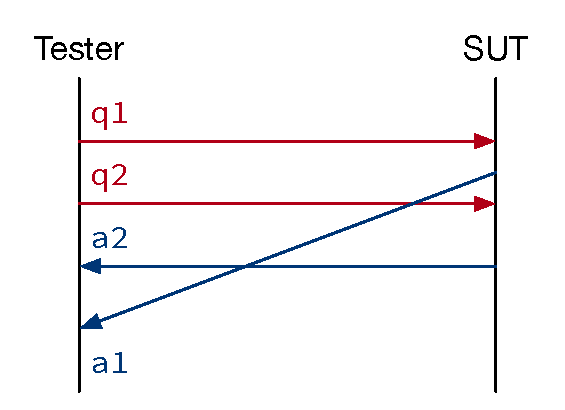
\includegraphics[width=\linewidth]{figures/ir-trace}
\end{minipage}
\caption{Labelled trace example.}
\label{fig:ir-trace}
\end{figure}

\begin{figure}
  \begin{minipage}[t]{.4\textwidth}
\begin{json}
  (* a2 = *)
  {
    "files": [
      {
        "name": "foo",
        "mode": 755
      },
      {
        "name": "bar",
        "mode": 500
      }
    ],
    "exitCode": 0
  }
\end{json}
  \end{minipage}\begin{minipage}[t]{.5\textwidth}
\begin{coq}
(* Jpath syntax defined in %\autoref{fig:ir-jexp}%. *)
Example second_file_mode: jpath :=
  this @ "files" # 2 @ "mode".

Example mode_add_write (j: IR) : IR :=
  match j with
  | JSON_Number n =>
    JSON_Number (mode_bits_or 200 n)
  | _ => j
  end.

Example id (j: IR) : IR := j.
\end{coq}
  \end{minipage}
  \caption{IR, Jpath, and heuristics function example.}
  \label{fig:ir-jpath}
\end{figure}

\paragraph{Syntax}
The J-expression is an extension of JSON that can encode trace-based heuristics.
As shown in \autoref{fig:ir-jexp}, a Jexp may include syntax
$(\Label.\Jpath.\Function)$ that represents trace-based heuristics, specified as:
\begin{enumerate}
\item The test harness records the trace as a list of labelled messages, where
  the requests are labelled odd, and their responses are labelled as the next
  even number.  The $\Label$ in a Jexp locates the IR in the trace with which
  the heuristics computes the input.  Labelling messages allows the reproducing
  trace-based heuristics despite shrinking and inter-execution nondeterminism.

  For example, consider the trace in \autoref{fig:ir-trace}: If a trace-based
  heuristics is interested in \ilc{q2}'s response \ilc{a2}, then it can be
  encoded as ``compute the test input based on message labelled 4'':
\begin{coq}
  Context get_label: labelT -> traceT -> IR.

  Compute get_label 4 labelled_trace.
  (* = a2 : IR *)
\end{coq}
  
  Suppose the test input is shrunk by removing \ilc{q1}, the label for \ilc{q2}
  remains unchanged as 3, so label 4 corresponds to the new response to
  \ilc{q2}:
\begin{coq}
  Example new_trace: traceT :=
    [(3, q2); (4, a2')].

  Compute get_label 4 new_trace.
  (* = a2' : IR *)
\end{coq}

As a result, the trace-based heuristics are preserved and adapted to new
executions during the shrinking process.
\item The $\Jpath$ is a path in the IR's syntax tree, and refers to a
  substructure of the IR that the heuristics uses.

  For example, suppose request \ilc{q2} lists files in a directory using the
  POSIX \inlinec{ls} command, and its response \ilc{a2} is encoded as the IR
  shown in \autoref{fig:ir-jpath}.  The response IR is a JSON object whose
  \inlinec{"files"} field is an array of objects, each has a \inlinec{"name"}
  and a \inlinec{"mode"} field.  A heuristic can refer to the second file's
  mode bits by Jpath \ilj{(this@"files"#2@"mode")}, which will guide the test
  harness to locate its corresponding value:
\begin{coq}
  Context get_jpath: jpath -> IR -> IR.

  Compute get_jpath second_file_mode a2.
  (* = JSON_Number 500 : IR *)
\end{coq}
\item The $\Function$ has type $(\mathsf{IR}\to\mathsf{IR})$, and defines the
  computation based on the sub-IR located by the Jpath.

  Consider the mode bits located in the previous example: If the heuristic
  wants to add write permission to the mode bits, it can do so with the
  \ilc{mode_add_write} function in \autoref{fig:ir-jpath}, which produces mode
  700.  Some heuristics might use the sub-IR 500 as-is, using the identity
  function \ilc{id}.
\end{enumerate}

\paragraph{Semantics}
J-expression provides a generic interface for test developers to implement
trace-based heuristics.  For the aforementioned file system example, the tester
can generate a request that changes the mode bits of an observed file, with the
following Jexp:
\begin{json}
  (* e5 = *)
  {
    "command": "chmod",
    "args": [
      4.(this@"files"#2@"mode").mode_add_write,
      4.(this@"files"#2@"name").id
    ]
  }
\end{json}

To instantiate Jexps into request IR, the test harness substitutes all
occurences of $(\Jref{l}{p}{f})$ in the Jexp with its corresponding IR computed
from the runtime trace:
\begin{coq}
  Definition eval (l: labelT) (p: jpath) (f: IR -> IR) (t: traceT) : IR :=
    let a: IR := get_label l t in
    let j: IR := get_jpath p a in
    f j.
\end{coq}

For example, given the runtime trace in \autoref{fig:ir-trace}, with \ilc{a2} is
defined in \autoref{fig:ir-jexp}, the the above Jexp is instantiated into the
following request:

\begin{json}
  (* instantiate e5 labelled_trace = *)
  { 
    "command": "chmod",
    "args": [ 700, "bar" ]
  }
\end{json}

However, when rerunning the test, the \ilc{new_trace} has a different response
associated with label 4.  The new response \ilc{a2'} might have fewer than 2
files in its payload.  Moreover, the response \ilc{a2'} might have not appeared
in the trace, due to delays in the environment.

To instantiate the original Jexp in such situations, I loosen the
\ilc{get_jpath} and \ilc{get_label} functions when evaluating the heuristics:
\begin{enumerate}
\item When evaluating a Jpath starting with \ilj{p#n}, if \ilj p corresponds to
  an array with fewer than \ilj n elements, or the array's \ilj n-th element
  cannot properly evaluate the remaining path, then try continuing the
  evaluation with any other element in the array.

  For example, consider evaluating \ilj{(this@3#"bar")} on the following IR's:
  \begin{center}
\begin{minipage}[t]{.5\linewidth}
\begin{json}
  (* j2 = *)
  [
    { "foo": 21 },
    { "bar": 22 }
  ]
\end{json}
\end{minipage}\begin{minipage}[t]{.5\linewidth}
\begin{json}
  (* j3 = *)
  [
    { "bar": 31 },
    { "baz": 32 },
    { "foo": 33 }
  ]
\end{json}
\end{minipage}
  \end{center}

  Here \ilj{j2} doesn't have a third element, and \ilj{j3}'s third element
  doesn't have field \ilj{"bar"}.  In these cases, \ilj{get_jpath} chooses other
  elements in the two arrays, resulting in value \ilj{22} for \ilj{j2}, and
  \ilj{31} for \ilj{j3}.
  
\item When evaluating label \ilj l and Jpath \ilj p on a trace, if the message
  labelled \ilj l does not exist in the trace, or cannot evaluate Jpath \ilj p
  properly, then try continuing the evaluation with any other IR in the trace.

  For example, consider evaluating J-expression \ilj{6.(this#2@"foo").id} on the
  following traces:
\begin{coq}
  Definition t1: traceT :=
    [(1,q1); (2,j2); (5,q2)].

  Definition t2: traceT :=
    [(3,q1); (4,j3); (5,q2); (6,a2)].
\end{coq}

Here \ilj{t1} doesn't have a message labelled 6, probably caused by environment
delays; \ilj{t2} has label 6 but its corresponding message is an object rather
than an array expected by the Jexp.  In these cases, \ilc{eval} chooses other
messages in the trace to evaluate, resulting in value \ilc{21} for \ilc{t1}, and
\ilc{33} for \ilc{t2}.
\end{enumerate}

By introducing loose evaluation of J-expressions, my test harness allows partial
instantiation of heuristics when the runtime trace is less than satisfying.

So far I have shown how to generate and shrink interactive test inputs and
address inter-execution nondeterminism.  In the next chapter, I'll combine this
test harness design with the validator practice in \autoref{chap:practices}, and
evaluate these techniques by testing real-world systems like HTTP servers and
file synchronizers.


\lys{Under construction:}

The IR in this framework is JSON, which allows syntax trees to be arbitrarily
wide and deep, and provides sufficient flexibility for network protocols in
general.  The J-expression is an extension of JSON that can refer to specific
fields in the trace:

The extended syntax
``$\Jref{\mathit{label}}{\mathsf{Jpath}}{\mathit{function}}$'' is a symbolic
expression that, given a runtime trace, can compute an IR of the request.  For
example, J-expression
``$\Jref{3}{\This\At\mathtt{"orders"}\Number2}{\mathtt{id}}$'' can be
pronounced: ``Look at the message labelled 3 in the trace, its `order' field
should be an array.  Find the 2nd element in that array, and use it
\ilc{id}entically (as-is).''  Such representation enables the test harness to
shrink counterexamples (encoded in Jexp) in a protocol-independent way.


\begin{figure}
  \begin{lstlisting}[style=customcoq]
    Example response1 : http_response :=
      Response (Status (Version 1 1) 200 (Some "OK"))
               [Field "ETag" "tag-foo";
                Field "Content-Length" "11"]
               (Some "content-bar").

    Example response2 : store_response :=
      Response__ListOrders [(233, (12, 100, 34, 500));
                            (996, (56, 400, 78, 20))].
  \end{lstlisting}
  \begin{minipage}[t]{.4\textwidth}
    \begin{lstlisting}[style=json]
      {
        "version": {
          "major": 1,
          "minor": 1
        },
        "code": 200,
        "reason": "OK",
        "fields": {
          "ETag": "tag-foo",
          "Content-Length": "11"
        },
        "body": "content-bar"
      }
    \end{lstlisting}
  \end{minipage}%
  \begin{minipage}[t]{.4\textwidth}
    \begin{lstlisting}[style=json]
      {
        "code": 200,
        "orders": [
          {
            "ID": 233,
            "BuyerID": 12,
            "BuyAmount": 100,
            "SellerID": 34,
            "SellAmount": 500
          },
          {
            "ID": 996,
            "BuyerID": 56,
            "BuyAmount": 400,
            "SellerID": 78,
            "SellAmount": 20
          }
        ]
      }
    \end{lstlisting}
  \end{minipage}
  \caption{Application message example for HTTP and online store protocols, and
    their corresponding intermediate representation}
  \label{fig:ir}
\end{figure}

To represent the correspondence between requests and responses, the trace labels
each message, and the request-response pair have the same label.
\autoref{fig:trace} shows a trace of messages sent and received by the tester
client.

\begin{figure}
  \begin{minipage}{.5\textwidth}
    \begin{lstlisting}[style=json]
      [
        {
          "label": 10,
          "message": {
            "method": "GET",
            "path": "index.html"
          }
        },
        {
          "label": 20,
          "message": {
            "method": "DELETE",
            "path": "index.html"
          }
        },
        {
          "label": 20,
          "message": {
            "code": 204,
            "reason": "No Content",
          }
        },
        {
          "label": 10,
          "message": {
            "code": 410,
            "reason": "Gone"
          }
        }
      ]
    \end{lstlisting}
  \end{minipage}%
  \begin{minipage}{.5\textwidth}
    \includegraphics[width=\textwidth]{figures/trace}
  \end{minipage}
  \caption{Example client-side trace and its corresponding IR}
  \label{fig:trace}
\end{figure}

\section{Instantiating requests during runtime}
To instantiate a Jexp into request IR, the test harness substitutes all
occurences of ``$\Jref{\mathit{label}}{\mathsf{Jpath}}{\mathit{function}}$''
with its corresponding IR computed from the trace.  However, due to external
nondeterminism, the expected message label might be delayed and not available in
the trace.  Also, considering inter-execution nondeterminism, arrays in observed
messages might not have enough elements as expected in the Jexp.  In these
cases, the test harness searches for other labels in the trace and other
elements in the arrays as a fallback fulfillment to construct the request.

\lys{Todo: add instantiation algorithm.}

This idea of shrinking symbolic representations can be applied to scenarios
beyond networked servers.  For example, the HTTP testing experiment in
\autoref{sec:eval} has also used this technique to locate the bug pattern.


\chapter{Evaluation}
\label{chap:eval}
This chapter evaluates the testing methodology presented in this thesis, by
deriving testers from specifications and running them against systems under
test.  

I conduct the experiments on two kinds of systems, \http server
(\autoref{sec:http}) and file synchronizer (\autoref{sec:sync}).  The research
questions are: (1) Qualitative: Is the tester useful to finding invalid behavior
in the SUT? and (2) Quantitative: Can the tester reveal those invalid behavior
quickly?

\section{Testing Web Servers}
\label{sec:http}

This thesis is motivated by the Deep Specification project~\cite{deepspec},
whose goal is to build systems with rigorous guarantee of functional
correctness, studying HTTP as an example.  I formalized a subset of \http
specification, featuring WebDAV requests GET, PUT, and POST~\cite{rfc4918}, ETag
preconditions~\cite{rfc7232}, and forward proxying~\cite{rfc7231}.

From the protocol specification written as ITrees, I derived a tester client
that sends and receives network packets.  \autoref{sec:http-sut} explains the
system under test and the experiment setup.  \autoref{sec:http-qual} and
\autoref{sec:http-quant} then describe the evaluation results qualitatively and
quantitatively.

\subsection{Systems Under Test}
\label{sec:http-sut}
I ran the derived tester against three server implementations:

\begin{itemize}
\item Apache HTTP Server~\cite{Apache}, which is among the most popular servers
  on the World Wide Web~\cite{http-netcraft,http-stats}.  I used the latest
  release 2.4.46, and edited its configuration file to enable WebDAV and proxy
  modules.
\item Nginx~\cite{nginx}, the other most popular server.  The experiment was
  conducted on the latest release 1.19.10, with only WebDAV module enabled,
  because Nginx doesn't fully support forward proxying like Apache does.
\item DeepWeb server developed in collaboration with \citet{itp21}, supporting
  GET and POST requests.  The server's functional correctness was formally
  verified, showing our methodology of specifying systems in testable and
  verifiable ways.
\end{itemize}

The tests were performed on a laptop computer (with Intel Core i7 CPU at 3.1
GHz, 16GB LPDDR3 memory at 2133MHz, and macOS 10.15.7).  The Apache and Nginx
servers were deployed as Docker instances, using the same host machine as the
tester runs on.  Our simple server was compiled into an executable binary, and
also ran on localhost.

The tester communicates with the server via POSIX system calls, in the same way
as over Internet except using address \inlinec{127.0.0.1}.  The round-trip time
(RTT) of local loopback is $0.08\pm0.04$ microsecond (at 90\% confidence).

\subsection{Qualitative Result}
\label{sec:http-qual}
\paragraph{Apache}
My tester rejected the Apache HTTP Server, which uses strong comparison for PUT
requests conditioned over \inlinec{If-None-Match}, while RFC~7232 specified that
\inlinec{If-None-Match} preconditions must be evaluated with weak comparison.
\bcp{What are strong and weak comparison?  \lys{ETag jargons.}}  I reported this
bug to the developers, and figured out that Apache was conforming with an
obsoleted \http standard~\cite{rfc2616}.  The latest standard has changed the
semantics of \inlinec{If-None-Match} preconditions, but Apache didn't update the
logic correspondingly.

To further evaluate the tester's performance in finding other violations, I
fixed the precondition bug by deleting 13 lines of source code and recompiling
the container.

The tester accepted the fixed implementation, which can be explained in two
ways: (1) The server now complies with the specification, or (2) The server has
a bug that the tester cannot detect.  To provide more confidence that (1) is the
case, I ran the tester against servers with known bugs, created by mutating the
Apache source code manually.\footnote{I didn't use automatic mutant generators
  because (i) Existing tools could not mutate all modules I'm interested in; and
  (ii) The automatically generated mutants could not cause semantic violations
  against my protocol specification.}

The tester rejected all 20 bugs, located in various modules of the Apache
server: \inlinec{core}, \inlinec{http}, \inlinec{dav}, and \inlinec{proxy}.
They appear both in control flow ({\it e.g.}, early return of handler function,
skipped precondition check) and in data values ({\it e.g.}, calling functions
with wrong parameters, flipping bits in computations, accessing buffer off by
one byte).  Some mutants took the tester longer time to reveal than others,
which will be discussed in \autoref{sec:http-quant}.

\paragraph{Nginx}
When testing Nginx, I found that its WebDAV module did not check the
\inlinec{If-Match} and \inlinec{If-None-Match} preconditions of PUT requests.  I
then browsed the Nginx bug tracker and found a ticket opened by
\citet{nginx242}, reporting the same issue with \inlinec{If-Unmodified-Since}
preconditions.

This issue has been recognized by the developers in 2016 but never resolved.
One possible reason is that the current architecture of Nginx makes it difficult
for the WebDAV module to utilize the precondition checker in the HTTP core
module.

A fix to this bug would involve either restructuring the modules or copying
source code from one module to another, unlike simply removing bad code in
Apache, so I only tested mutants for the latter.

\paragraph{DeepWeb}
My test derivation framework was developed in parallel with the DeepWeb server.
After my collaborators finished the formal proof of the server's functional
correctness, I tested the server with my derived tester.  The tester has
revealed a liveness issue---when a client pipelines more than one requests in a
single connection, the server may hang without processing the latter requests.

This liveness bug was out of scope for the server's functional correctness,
which only requires the server not to send invalid messages.  Such partial
correctness may be trivially satisfied by a silent implementation that never
responds.  My experiments has shown this limitation in formal verification, and
guided the debugging of the server implementation.

These results show that my tester is capable of finding different kinds of bugs
in server implementations, within and beyond functional correctness.  Next I'll
evaluate how long the tester takes to reveal bugs.

\lys{Under construction:}

\subsection{Quantitative Result}
\label{sec:http-quant}

\begin{figure*}
  
\includegraphics[width=\textwidth]{figures/http-time}
  \caption[Cost of detecting bug in each server/mutant.]{Cost of detecting bug
    in each server implementation.  The left box with median line is the
    tester's execution time before rejecting the server, which includes
    interacting with the server and checking its responses.  The right bar with
    median circle is the number of \http messages sent and received by the
    tester before finding the bug.  Results beyond 25\%--75\% are covered by
    whiskers.
    %% \bcp{The red horizontal
    %%   lines are very confusing: make them blue!  Also, we need to explain
    %%   what all the parts of the figure mean (or, better, remove most of
    %%   them!)---the thin dotted parts, thin solid parts, why the dotted ones
    %%   are terminated and the solid ones are not, ...}
  }
  \label{fig:checker-performance}
\end{figure*}

To answer Research Question (2) at the beginning of this chapter, I measure the
execution time and network interactions taken to reject vanilla Apache and its
mutants, as shown in \autoref{fig:checker-performance}.  The 20 mutants are
named after the module where I inserted the bug.  The tester rejected all the
buggy implementations within 1 minute, and in most cases, within 1 second.  This
does not include the time for shrinking the counterexample.

Some bugs took longer time to find, and they usually required more interactions
to reveal.  This may be caused by (1) The counter-example has a certain pattern
that my generator didn't optimize for, or (2) The tester did produce a
counter-example, but failed to reject the wrong behavior.  I determine the real
cause by analyzing the bugs and their counterexamples:

\begin{figure}
  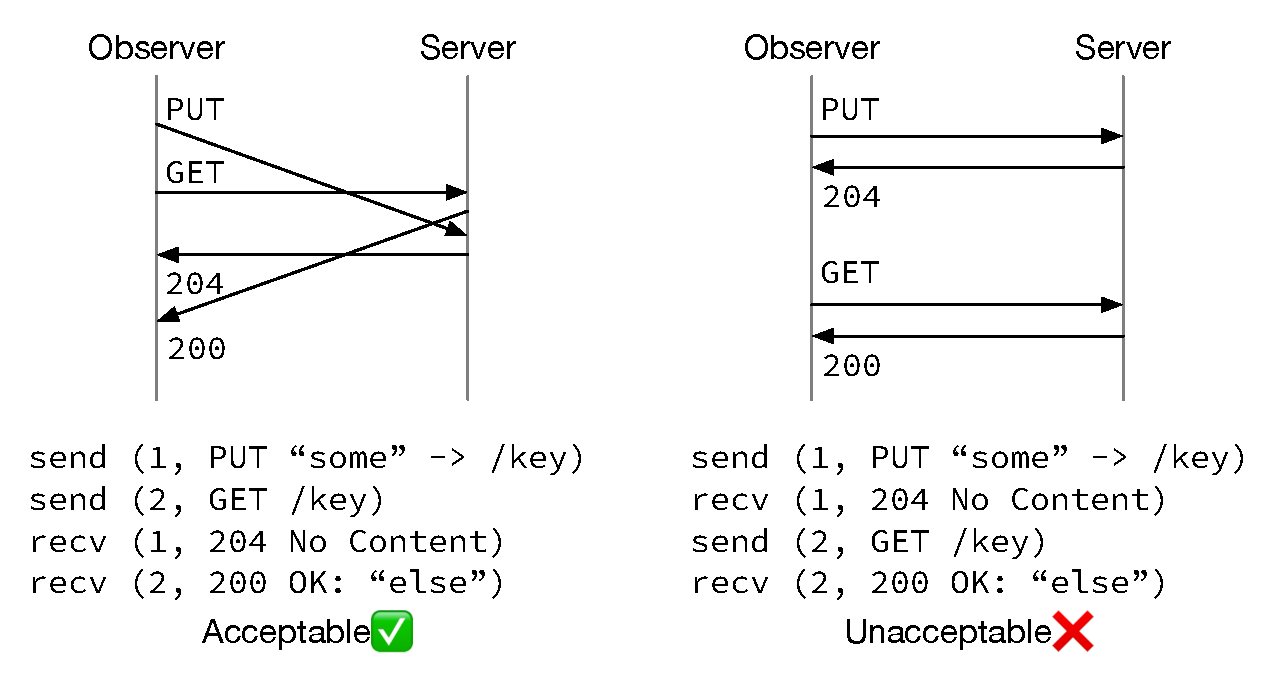
\includegraphics[width=\linewidth]{figures/http-put-bug}
  \caption[GET-after-PUT bug pattern in Apache mutants.]{GET-after-PUT bug
    pattern in Apache mutants.  The trace on the left does not convince the
    tester that the server is buggy, because there exists a certain network
    delay that explains why the PUT request was not reflected in the 200
    response.  When the trace is ordered as shown on the right, the tester
    cannot imagine any network reordering that causes such observation, thus
    must reject the server.}
  \label{fig:put-bug}
\end{figure}
  
\begin{itemize}
  \item Mutants 19 and 20 are related to the WebDAV module, which handles PUT
    requests that modify the target's contents.  The buggy servers wrote to a
    different target from that requested, but responds a successful status to
    the client.

    The tester cannot tell that the server is faulty until it queries the
    target's latest contents and observes an unexpected value.  To reject the
    server with full confidence, these observations must be made in a certain
    order, as shown in \autoref{fig:put-bug}.

  \item Mutant 18 is similar to the bug in vanilla Apache: the server should
    have responded with 304 Not Modified, but sent back 200 OK instead.  To
    reveal such violation, a minimal counterexample consists of 4 messages:
    \begin{enumerate}
    \item GET request,
    \item 200 OK response with some ETag \inlinec{"x"},
    \item GET request conditioned over \inlinec{If-None-Match: "x"}, and
    \item 200 OK response, indicating that the ETag \inlinec{"x"} did not match
      itself.
    \end{enumerate}
    Notice that (2) must be observed before (3), otherwise the tester will not
    reject the server, with a similar reason as \autoref{fig:put-bug}.

  \item Mutant 5 causes the server to skip some code in the core module, and
    send nonscence messages when it should respond with 404 Not Found.  The
    counterexample can be as small as one GET request on a non-existential
    target, followed by a non-404, non-200 response.  However, my tester
    generates request targets within a small range, so the requests' targets are
    likely to be created by the tester's previous PUT requests.

    Narrowing the range of test case generation might improve the performance in
    aforementioned Mutants 18--20, but Mutant 5 shows that it could also degrade
    the performance of finding some bugs.

  \item The mutants in proxy module caused the server to forward wrong requests
    or responses.

    To test servers' forward proxying functionality, the tester consists of
    clients and origin servers, both derived by dualization.  When the origin
    server part of the tester accepts a connection from the proxy, it does not
    know for which client the proxy is forwarding requests.  Therefore, the
    tester needs to check the requests sent by all clients, and make sure none
    of them matches the forwarded proxy request.

    The more client connections the tester has created, the longer it takes the
    tester to check all connections before rejecting a buggy proxy.
\end{itemize}

These examples show that the time-consuming issue of some mutants are likely
caused by the generators' heuristics.  Cases like Mutant 5 can be optimized by
state-based heuristics in \autoref{sec:heuristic-state}; Proxy-related bugs can
be more easily found by trace-based heuristics in \autoref{sec:heuristic-trace};
For Mutants 18--20, the requests should be sent at specific time periods so that
the resulting trace is unacceptable per specification, which is discussed in
\autoref{chap:discussion}.

\section{Testing file synchronizer}
\label{sec:sync}

To demonstrate the generality of my specification-based testing methodology, I
applied it to file synchronizers.  \autoref{sec:file-sut} introduces my
specification of the file system and synchronization semantics.  From these
specifications, I derived a tester program for the Unison file
synchronizer~\cite{unison}, with results shown in \autoref{sec:file-result}.

\subsection{System Under Test}
\label{sec:file-sut}
A file synchronizer manipulates the file system to reconcile updates in
different replicas~\cite{what-sync}.  To check a synchronizer's correctness, the
tester needs to update replicas, launch the synchronization process, and observe
the propagated updates.

\begin{figure}
\begin{coq}
  Inductive node :=
    File      : content          -> node
  | Directory : list (name*node) -> node.

  Context read : path -> node    -> option content.
  Context write: path -> content -> node -> option node.
  Context mkdir: path -> node    -> option node.
  Context ls   : path -> node    -> list name.
  Context rm   : path -> node    -> option node.
\end{coq}
\caption{File system specification.}
\label{fig:file-spec}
\end{figure}

My specification consists of two parts:
\begin{enumerate}
  \item A file system model represented as a tree, where the leaves are files
    and the branches are directories.  As shown in \autoref{fig:file-spec}, the
    file system model is a simplified abstraction from the POSIX file interface,
    ignoring metadata and file permissions.  Specifying more aspects of the file
    system is discussed in \autoref{chap:discussion}.

    Based on the file system model, I specified five basic file operations
    the tester may perform: (i) reading contents from a file, (ii) writing
    contents to a file, (iii) creating a new directory, (iv) listing entries
    under a directory, and (v) removing a file or directory recursively.

    Some file operations may fail {\it e.g.} when reading from a path that
    refers to a directory.  These failures are represented as return value
    \ilc{(None: option _)} in the node functions.
  \item A file synchronizer model that syncs updates between two replicas,
    implementing the reconcilation algorithm by \citet{what-sync}:
\begin{coq}
  Definition sigma := node*node*node.
      
  Context reconcile: sigma -> sigma.
\end{coq}
Notice that the \ilc{reconcile} function manipulates three replicas.  This is
because the synchronizations might be partial: Upon write-write and write-delete
conflicts, the synchronizer does not propagate the conflicting updates, and
leaves the dirty files untouched in both replicas.

The third parameter of the reconcile function represents the subset of the two
replicas that were synchronized: \ilc{(reconcile (a,b,g))} syncs replicas \ilc a
and \ilc b based on their previous consensus \ilc g.  The consensus is initially
empty, and updated when a change in one replica is propagated to another, or the
two replicas have made identical changes.
\end{enumerate}

\begin{figure}
\begin{coq}
  Variant F :=        (* file operations *)
  Fls    (p: path)
| Fread  (p: path)
| Fwrite (p: path) (c: content)
| Fmkdir (p: path)
| Frm    (p: path).

Variant R := R1 | R2. (* replicas      *)

Variant Q :=          (* query type    *)
  QFile (r: R) (f: F)
| QSync.

Variant A :=          (* response type *)
  Als   (l: list name)
| Aread (c: content)
| Aexit (z: Z).       (* exit code     *)
\end{coq}
\caption{Query and response types for testing file synchronizer.}
\label{fig:file-type}
\end{figure}

Having specified the file system interface and the reconcilation semantics, I
modelled the SUT as a deterministic QA server described in
\autoref{def:qaserver}.  As shown in \autoref{fig:file-type}, the request type
\ilc Q can be file operations or the synchronization command; the response type
\ilc A carries the return value of file system queries, or the transactions'
exit code.  For example, when synchronizing the two replicas, code 1 indicates
partial synchronization with conflicts unresolved, and code 2 means the
synchronizer has crashed due to uncaught exceptions or interruptions.

The QA model for the file system+synchronizer was dualized into a tester program
that makes system calls to manipulate files, launch the synchronizer, and
observe the updates.  The system calls are made one at a time, and the file
synchronizer is run as a foreground process that blocks other interactions.
Testing the synchronizer as a nonblocking background process is discussed in
\autoref{chap:discussion}.

\subsection{Experiment Results}
\label{sec:file-result}
The tester has revealed two features of the Unison file synchronizer, and I
reported them to the developers.  By analyzing the program's behavior, the
developers determined that Unison did not violate its specification, which
allows a wider set of behavior than my specification defines.  The revealed
features are as follows:

\paragraph{Synchronizing read-only directories}
When the tester creates a directory in one replica with read and execution
permission (mode \ilj{500}) and calls the synchronization command, Unison
crashed without creating the corresponding directory in the other replica.

The crashing behavior only occurs on macOS, and is caused by Unison's mechanism
for propagating changes: When copying directory \ilj{foo} from replica \ilj A to
replica \ilj B, the synchronizer first creates a temporary directory
``\ilj{B/.unison.foo.xxxx.unison.tmp}'', and then renames it to ``\ilj{B/foo}''.
The \inlinec{rename} implementation in macOS requires write permission to
proceed, so the change was not propagated.

This issue is not considered a violation in Unison or macOS, because: (1) Unison
is allowed to halt without propagating an expected change, as long as its exit
code has indicated an error, and no unexpected change was propagated.  (2) The
POSIX specification~\cite{posix} says the \inlinec{rename} function {\it may}
require write access to the directory.

Despite being compliant to the specification, this feature in Unison is
considered a defect, as it disables synchronization of read-only files and
directories.  A potential fix might be substituting \inlinec{rename} with other
system calls.

This defect was revealed by accident: My file system specification in
\autoref{fig:file-spec} does not mention file permissions, so I defaulted to
mode \ilj{755}.  However, when implementing the test executor, I made a typo
that wrote the permission as hexadecimal \ilc{0x755} while it should be octal
\ilc{0o755}.  This caused the created directory to have mode bits \ilj{525},
which triggered the aforementioned behavior.

This experiment shows that my current abstraction of the file system is worth
expanding to include more information like file permissions, which might reveal
other features of the file synchronizer.

The experiment also reveals a challenge in specifying programs, that the
underlying operating system might also pose uncertainty to the program's
behavior.  Such external nondeterminism may be handled by parameterizing the
program's specification over the OS's, in a similar way as composing the server
model with the network model in \autoref{sec:external-nondet}.


\chapter{Related Work}
\label{chap:related-work}
This chapter explores methodologies in specifying and automatically testing
interactive systems.
\autoref{sec:related-validate} compares different specification
techniques for testing purposes.
\autoref{sec:related-harness} then discusses practices in developing test
harnesses.

\section{From Specifications to Validators}
\label{sec:related-validate}

Different testing scenarios exhibit various challenges that motivate the
specification design.  This section partitions the validation techniques by the
languages used for developing the specifications.

\subsection{State machine specification: Quviq QuickCheck}
Property-based testing with QuickCheck has been well adopted in industrial
contexts~\cite{Hughes2016}.  The specification is a boolean function over traces
{\it i.e.} the validator.  My solutions to addressing internal and external
nondeterminism are inspired by practices in QuickCheck.

\paragraph{Internal nondeterminism}
My \http specification was initially written as a QuickCheck property.  Before
handling preconditions like \inlinec{If-Match} and \inlinec{If-None-Match}, the
validator implements a deterministic server model and compares its behavior with
the observations, as shown in the \ilc{validate} function in
\autoref{sec:interactive-testing}.  When expanding the specification to cover
conditional requests, I implemented the ad hoc validator by manually translating
the trace into tester-side knowledge, as shown in \autoref{fig:etag-tester}.

The complexity in describing ``what behavior is valid'' motivated me to rephrase
the specification.  I applied the idea of model-based
testing~\cite{broy2005model}, and specified the protocol in terms of ``how to
produce valid behavior''.  My specification represented internal nondeterminism
with symbolic variables.  The validator then checks whether the trace is
producible by the symbolic specification, by reducing the producibility problem
to constraint solving.

\paragraph{External nondeterminism}
\citet{testing-dropbox} have used QuickCheck to test Dropbox.  The specification
does not involve internal nondeterminism, but does handle external
nondeterminism that local nodes may communicate with the server at any time.
This is done by introducing ``conjectured events'' to represent the possible
communications.  The validator checks if the conjectured events can be inserted
to somewhere in the trace to make it producible by the model.

To specify servers' allowed observations delayed by the network, \citet{cpp19}
introduced the concept of ``network refinement''.  The network may scramble the
traces by delaying some messages after others, with one exception: If the client
has received response \ilc A before it sends request \ilc Q, then by causality,
the server-side trace must have sent response \ilc A before receiving request
\ilc Q.  Upon observing a client-side trace \ilc T, our QuickCheck validator
searches for a server-side trace that (i) can be reasonably scrambled into trace
\ilc T, and (ii) complies with the protocol specification.

My network model design in \autoref{sec:external-nondet} was inspired by these
ideas of conjecturing the environment's behavior.  Instead of inserting
conjectured communication events or reordering the trace, I specified the
network as an independent module and composed it with the server specification.
This provides more flexibility in specifying asynchronous systems: (i) To adjust
the network configurations, e.g., limiting the buffer size or the number of
concurrent connections, we only need to adjust the network model without
modifying the server's events.  (ii) Instead of carefully defining the space of
valid scrambled traces for each network configuration, we can derive it from the
network model by dualization.  (iii) The network model is reusable and allows
specifying various protocols on top of it.

\subsection{Process algebra: LOTOS and TorXakis}
Language of Termporal Ordering Specification (LOTOS)~\cite{lotos} is the ISO
standard for specifying OSI protocols.  It defines distributed concurrent
systems as {\em processes} that interact via {\em channels}.  Using a formal
language strongly inspired by LOTOS, \citet{torxakis-dropbox} implemented a test
generation tool called TorXakis, and used it for testing Dropbox.

TorXakis supports internal nondeterminism by defining a process for each
possible value.  This requires the space of invisible values to be finite.  In
comparison, I represented invisible values as symbolic variables and employed
constraint solving that can handle inifitite space of data like strings and
integers.

As for external nondeterminism, TorXakis hardcodes all channels between each
pair of processes, assuming no new process joins the system.  Whereas in my
network model, ``channels'' are the ``source'' and ``destination'' fields of
network packets, which allows specifying a server that exposes its port to
infinitely many clients.

\subsection{Transition systems: NetSem and Modbat}
Using labelled transition systems (LTS), \citet{netsem} have developed rigorous
specification for TCP, UDP, and the Sockets API.  To handle internal
nondeterminism in real-world implementations, they symbolized the model states,
which is then evaluated with a special-purpose model symbolic model checker.
The tester helped revealing their post-hoc specifications' mismatch with
mainstream systems like FreeBSD, Linux, and WinXP.  I borrowed the idea of
symbolic evaluation in validating observations, and used it for detecting
mainstream servers' violations against the formalized RFC specification.

\citet{modbat} have generated test cases for Java network API, which involves
blocking and non-blocking communications.  Their abstract model was based on
extended finite state machines (EFSM), and could capture bugs in the network
library \verb|java.nio|.  Their validator rejects the SUT upon unexpected
exceptions or observations that fail its {\em encoded} assertions.  In
comparison, assertions in my validator are {\em derived} from the abstract
model, which covers full functional correctness of the SUT modulo external
nondeterminism.

\section{Test Harnesses}
\label{sec:related-harness}
This section explores techniques of generating and shrinking test inputs.
\autoref{sec:related-gen} compares different heuristics used by test generators;
\autoref{sec:related-shrink} explains existing shrinking techniques for
interactive testing scenarios.

\subsection{Generator Heuristics}
\label{sec:related-gen}

In addition to state-based and trace-based heuristics discussed in
\autoref{sec:heuristics}, other kinds of heuristics can be applied to generating
inputs for various testing scenarios.

\paragraph{Constraint-based heuristics}
The reason for introducing heuristics is to increase the chance of triggering
invalid behavior.  I specified the heuristics as ``how to produce interesting
input'', while in some cases, it's more convenient to specify ``what inputs are
interesting''.  For example, well-typed lambda expressions can be easily defined
in terms of typing rules, but are less intuitive to enumerate by a generator.

Narrowing~\cite{narrowing} allows generating data that satisfy certain
constraints.  \citet{gengood} have applied the idea of narrowing to the
QuickChick testing framework in Coq~\cite{quickchick}, representing constraints
as inductive relations.  The relations are compiled into efficient generators
that produce satisfying data.

The narrow-based generator in QuickChick has been used during my preliminary
experiment with \http, where I defined a well-formed relation for HTTP requests
to guide the generator.  However, the QuickChick implementation was unstable and
failed to derive generators as my type definition becomes more and more complex.
This constraint-based heuristics may be integrated to my current testing
framework by interpreting QuickChick's \ilc{Gen} (generator) monad into
the \ilc{IO} monad used by the test harness, provided the generator derivation
failure gets resolved.

\paragraph{Coverage-based heuristics}
Another strategy to increase the chance of revealing invalid behavior is to
cover more execution paths of the SUT.  This idea is applied to fuzz
testing~\cite{fuzz}, with popular implementations AFL~\cite{afl} and
Honggfuzz~\cite{honggfuzz}, and combined with property-based testing by
\citet{fuzzchick}.

Coverage-based testers mutate the test inputs and observe the programs'
execution paths.  An input is considered interesting if it causes the program to
traverse a previously unvisited path.  The interesting inputs will be mutated
and rerun to cover potentially more paths.

To track the program's execution paths, coverage-based heuristics need to
instrument the SUT during compilation, making it inapplicable for black-box
testing.  When fuzzing interactive systems like web servers, the SUT is run in a
simulator where the requests are provided as files instead of network packets.
The responses are ignored by the comtemporary fuzzing tools, which only checks
whether the SUT crashes or hangs and does not care about functional correctness
like the responses' contents.  To produce a trace for validation, the SUT needs
to be carefully modified to record its send and receive events.  Addressing
these challenges would enable coverage-based heuristics to be integrated in
interactive testing of systems' functional correctness.

\subsection{Shrinking Interactive Tests}
\label{sec:related-shrink}

To address inter-execution nondeterminism in Quviq QuickCheck,
\citet{Hughes2016} introduced the idea of shrinking abstract representations of
test input.  The tester first generates a {\em script} using state-based
heuristics, and instantiates the script with the tester's runtime state.  The
scripts can be shrunk and adapted to new runtimes when rerunning the test.

The language design of my test harness is inspired by the QuickCheck approach,
and extends it in two dimensions:
\begin{enumerate}
\item The QuickCheck framework assumes synchronous interactions, where the
  requests are function calls that immediately return.  When testing
  asynchronous systems {\it e.g.} networked servers, the responses might be
  indefinitely delayed by the environment, which would block the QuickCheck
  tester's state transition.
  
  To generate test inputs asynchronously, I implemented a non-blocking algorithm
  for instantiating scripts into requests.  When a dependant observation is
  absent due to delays or loss by the environment, the test harness tries to
  instantiate the request using other observations, instead of waiting for the
  observation from the environment.

\item QuickCheck requires the test developer to specify a runtime state to guide
  the generator, and define the state transition rules for each interaction.
  The heuristics are implemented based on the tester's point of view.

  In comparison, my framework replaced these requirements with state- and
  trace-based heuristics, where the model state was exposed by the underlying
  specification, and the trace was automatically recorded by the test harness.
  This allows test developers to design heuristics based on the implementation's
  point of view, instead of reasoning on the implementation's internal and
  external nondeterminism based on its observations.
\end{enumerate}


\chapter{Discussions}
\label{chap:discussion}

\chapter{Conclusion}
\label{chap:conclusion}

\printbibliography
  %% ASZ: AucTeX (the Emacs package for LaTeX I used) doesn't support a `.bib`
  %% file and a `.tex` file with the same name

\appendix

\chapter{Mathematical Proof of Derived Validators' Correctness}
\label{chap:math-proof}
\section{Forward preservation lemma for rejection soundness}
\label{sec:rs2-proof}
\autoref{eq:rs2}

\begin{align*}
  &\forall(p:\Prog)(q,c,a:\Int)(s_0,s':\sigma)(v:\beta),\\
  &\sstep_p(q,c,s_0)=(a,s')\wedge\Reflects{v}{s_0}\\
  &\implies\exists v':\beta,\vstep_p(q,a,v)=\Some{v'}\wedge\Reflects{v'}{s'}
\end{align*}

The invariant $\Reflects{v}{s_0}$ tells us that $v$ contains a validation state
that reflects the server state $s_0$:
\[\exists((vs_0,cs_0)\in v)(asgn_0:\Var\to\Int),\satisfy{asgn_0} cs_0\wedge {vs_0}^{asgn_0}\equiv s_0\]

The corresponding validator step is constructed by analyzing the server step,
and proving small-step bisimulation for each derivation rule
in \autoref{sec:dualization}.

\paragraph{Write}
The server writes some expression $(e:\Sexp)$ to an address $!dst$.
According to \autoref{rule:write}, the validator creates a fresh variable $x_e$
for address $!dst$, and constraints that $(\#x_e\equiv e^{vs})$.\footnote{If
unspecified, $(vs,cs)$ represents the pre-small-step validator state, and $s$
represents the pre-small-step server state.}

We need to show that:
\begin{align*}
&\forall vs,cs,s,asgn,\\
&\satisfy{asgn}{cs}\wedge vs^{asgn}\equiv s\\
&\implies\forall d,e,\begin{array}[t]{lll}
\letin{s'&}{\update{s}{d}{e^s}&}\\
\letin{(vs',cs')&}{\Write(d,e,(vs,cs))&}\\
\multicolumn{3}{l}{\exists asgn',\quad\satisfy{asgn'}{cs'}\wedge vs'^{~asgn'}\equiv s'}
\end{array}
\end{align*}
\begin{proof}
Based on the definition of $\Write$, we need to show that:
\begin{align*}&\letin{x_e}{\Fresh(vs,cs)}\\
&\letin{vs'}{\update{vs}{d}{x_e}}\\
&\letin{cs'}{cs\cup\{x_e\equiv e^{vs}\}}\\
&\exists asgn',\quad\satisfy{asgn'}{cs'}\wedge vs'^{~asgn'}\equiv s'
\end{align*}
Let:\[asgn'=\update{asgn}{x_e}{e^{s}}\]

In order to prove $(\satisfy{asgn'}{cs'})$, we introduce some generic lemmas to
show that $(\satisfy{asgn'}{cs})$ and $({x_e}^{asgn'}\equiv{(e^{vs})^{asgn'}})$:
\begin{lemma}[Fresh variable preserves satisfaction]
\label{lem:fresh-sat}
\begin{align*}
&\forall (cs:\Set\constraint)(asgn:\Var\to\Int),\\
&\satisfy{asgn}{cs}\\
&\implies
\begin{array}[t]{lll}
\multicolumn{3}{l}{\forall (z:\Int),vs,}\\
\letin{x&}{\Fresh(vs,cs)&}\\
\letin{asgn'&}{\update{asgn}{x}{z}&}\\
\multicolumn{3}{l}{\satisfy{asgn'}{cs}}
\end{array}
\end{align*}
\begin{proof}
Since $x$ is fresh in $cs$, we have:
\[\forall (e_1\ccmp e_2)\in cs,\quad{e_1}^{asgn'}={e_1}^{asgn}\wedge{e_2}^{asgn'}={e_2}^{asgn}\]

Thus:
\begin{align*}
&\forall (e_1\ccmp e_2)\in cs,\quad{e_1}^{asgn'}\ccmp {e_2}^{asgn'}\\
&\textit{i.e. }\satisfy{asgn'} cs
\end{align*}
\end{proof}
\end{lemma}

\begin{lemma}[Fresh variable preserves evaluation]
\label{lem:fresh-eval}
\begin{align*}
&\forall (vs:\Nat\to\Var)(asgn:\Var\to\Int)(z:\Int),cs,\\
&\begin{array}[t]{lll}
\letin{x&}{\Fresh(vs,cs)&}\\
\letin{asgn'&}{\update{asgn}{x}{z}&}\\
\multicolumn{3}{l}{\forall (e:\Sexp),(e^{vs})^{asgn'}=(e^{vs})^{asgn}}
\end{array}
\end{align*}
\begin{proof}
Assume to the contrary that: \[(e^{vs})^{asgn'}\neq(e^{vs})^{asgn}\]

Since $asgn'$ is the same as $asgn$ except for variable $\#x$, we know that
$(e^{vs}:\Vexp)$ must involve $\#x$.  Therefore, $e$ must involve some address
$!k$ such that $(vs!k=x)$.  This contradicts the fact that $x$ is fresh in $vs$.
\end{proof}
\end{lemma}

\begin{lemma}[Symbolization preserves evaluation]
\label{lem:sym-eval}
\begin{align*}
&\forall(vs:\Nat\to\Var)(asgn:\Var\to\Int)(s:\Nat\to\Int),\\
&vs^{asgn}\equiv s\implies\forall (e:\Sexp),\quad(e^{vs})^{asgn}\equiv e^s
\end{align*}
\begin{proof}
Based on the definition of symbolization and evaluation:
\begin{itemize}
\item $e^{vs}$ substitutes all occurences of $!k$ in $e$ with $\#(vs!k)$;
\item $(e^{vs})^{asgn}$ substitutes all occurences of $\#(vs!k)$ to $asgn!(vs!k)$;
\item $e^s$ substitutes all occurences of $!k$ in $e$ with $(s!k)$.
\end{itemize}

From the hypothesis that $(vs^{asgn}\equiv s)$, we have:
\[\forall (k:\Nat),\quad asgn!(vs!k)\equiv (s!k)\]

Therefore, we know that all occurences of $!k$ were mapped to the same value
between the two evaluation paths.
\end{proof}
\end{lemma}

Based on \autoref{lem:fresh-eval}, we have:
\[{(e^{vs})}^{asgn'}={(e^{vs})}^{asgn}\]



Also, since $x_e$ is free in $vs$, and $asgn'$ is the same as $asgn$ except for
$x_e$, we have:
\[\forall k,asgn'!(vs'!k)=\begin{cases}
asgn'!x_e=e^s=(s'!k)&k\Is d\\
asgn!(vs!k)=(s!k)=(s'!k)&\text{otherwise}
\end{cases}\]
Therefore:\[vs'^{~asgn'}\equiv s'\]
\end{proof}

\paragraph{Havoc}
When the server writes some internal choice $c$ to address $d$,
according to \autoref{rule:choice}, the validator creates a fresh variable for
address $!d$.

We need to show that:
\begin{align*}&\forall vs,cs,s,asgn,\\
&\satisfy{asgn}{cs}\wedge vs^{asgn'}\equiv s\\
&\implies\forall d,c,\begin{array}[t]{lll}
\letin{s'&}{\update{s}{d}{c}&}\\
\letin{x_c&}{\Fresh(vs,cs)&}\\
\multicolumn{3}{l}{\exists asgn',\quad\satisfy{asgn'} cs\wedge vs^{asgn'}\equiv s'}
\end{array}
\end{align*}
\begin{proof}
Let:\[asgn'=\update{asgn}{x_c}{c}\]
Since $x_c$ is free in $cs$, we have
\end{proof}

%% \[\havoc(d,(vs,cs))=\letin{x_c}{\Fresh(vs,cs)}{(\update{vs}{d}{x_c},cs)}\]

%% \begin{proof}
%% We can construct the following assignment:
%% \[asgn_1=\update{asgn_0}{x_c}{c}\]


%% Since $x_c$ is also fresh in $vs_0$, we have:
%% \[\forall addr, asgn_1!(vs_1!addr)=\begin{cases}
%% asgn_1!x_c=c\equiv s_1!addr&addr\Is1\\
%% asgn_0!(vs_0!addr)=s_0!addr\equiv s_1!addr&\text{otherwise}
%% \end{cases}\]

%% Thus: \[{vs_1}^{asgn_1}\equiv s_1\]
%% \end{proof}

\section{Backward preservation lemma for rejection completeness}
\label{sec:rc2-proof}

\autoref{eq:rc2}


\chapter{Unstructured contents}
\section{Challenges: Testing Internal and Network Nondeterminism}
\label{sec:challenge}
To illustrate the challenges in testing networked applications, we discuss two
features of \http---conditional requests~\cite{rfc7232}
and message forwarding~\cite{rfc7231}---showcasing internal nondeterminism
and network nondeterminism, respectively.
%% \hzh{we should make sure we always use either internal/external or
%% internal/network. in particular, the 3rd contribution uses internal/external,
%% while everywhere else seems to use internal/network.}

\paragraph*{Internal Nondeterminsm}
\http requests can be conditional: if the client has a local copy of some
resource and the copy on the server has not changed, then the server needn't
resend the resource.  To
achieve this, an \http server may generate a short string, called an ``entity tag'' (ETag), identifying the
content of some resource, and send it to
the client: %% \bcp{Make the font a bit smaller}
\begin{lstlisting}[style=customc]
/* Client: */
GET /target HTTP/1.1

/* Server: */
HTTP/1.1 200 OK
ETag: "tag-foo"
... content of /target ...
\end{lstlisting}
The next time the client requests the same resource, it can include the ETag in
the GET request, informing the server not to send the content if its ETag
still matches:

\begin{lstlisting}[style=customc]
/* Client: */
GET /target HTTP/1.1
If-None-Match: "tag-foo"

/* Server: */
HTTP/1.1 304 Not Modified
\end{lstlisting}
% The server compares the request's ETag with that stored for the target
% resource.
% If matched, the server responds with code 304 and the client knows the
% target's
% content has not changed from the previously sent content.
If the tag does not
match, the server responds with code 200 and the updated content as usual.
%
Similarly, if a client wants to modify the server's resource atomically by
compare-and-swap, it can include the ETag in the PUT request as \inlinec{If-Match} precondition, which
instructs the server to only update the content if its current ETag matches.
% \begin{lstlisting}[style=customc]
% /* Client: */
% PUT /target HTTP/1.1
% If-Match: "tag-outdated"
%
% /* Server: */
% HTTP/1.1 412 Precondition Failed
% \end{lstlisting}
% The server compares the request's ETag with the target's.  If they don't match
% (indicating the client has an outdated version of the target resource), the
% server does not process the modification, and responds with code 412.  Only if
% the client provides a matching ETag does the server update the target's content
% per requested.  A pseudocode for this compare-and-swap logic is shown in
% \autoref{fig:if-match-model}.

\ly{This is a good example, but how general is the
  problem, since one might question the popularity of ETags? On the other hand,
  if your testing framework targets application layer protocols rather than just
  HTTP, maybe there are more similar examples? For example, file/mail servers or
  databases might also require some synchronization mechanisms similar to
  compare-and-swap? And there might be other examples that's not
  compare-and-swap?}\bcp{Agree that this is important to discuss.}
  \lys{Mentioned at the end of this section.}

Thus, whether a server's response should be judged {\em valid} or not
depends on the ETag it generated
when creating the resource.  If the tester doesn't know the server's internal
state ({\it e.g.}, before receiving any 200 response including the ETag), and
cannot enumerate all of them (as ETags can be arbitrary strings), then it needs
to maintain a space of all possible values, narrowing the space upon further
interactions with the server.
% ~\ly{If I understand it correctly, the
%   non-determinism mostly comes from the fact that the algorithm to generate
%   ETags is unknown and depends on a lot of server's internal states---the fact
%   that the server supports ``compare and swap'' seems less relevant? If so, I
%   think this subsection should focus more on where the non-determinism comes
%   from, and why this makes it hard for testers, rather than demonstrating how
%   HTTP/1.1 implements ``compare and swap''.}\bcp{I agree---the whole
%   compare-and-swap discussion could be reduced to a sentence.  I'll make
%   this fix.}

It is possible, but tricky, to write an ad hoc tester for \http by
manually ``dualizing'' the behaviors described by the informal specification
documents (RFCs).
The protocol document describes {\em how} a valid server should handle
requests, while the
tester needs to determine {\em what} responses received
from the server are valid.  For example, ``If the server has revealed some
resource's ETag as \inlinec{"foo"}, then it must not reject requests targetting
this resource conditioned over \inlinec{If-Match: "foo"}, until the resource has
been modified''; and ``Had the server previously rejected an \inlinec{If-Match}
request, it must reject the same request until its target has been
modified.'' \autoref{fig:etag-tester} shows a hand-written tester for
checking this bit of ETag functionality; we hope the reader will agree that
this testing logic is not straightforward to derive from the informal
``server's eye'' specifications.

\paragraph*{Network Nondeterminism}
%% \lys{Network nondeterminism seems more important as a contribution, but internal
%%   nondeterminism were discussed much more.}\sz{Maybe drop the subsection and
%%   call out ``internal'' vs. ``network'' nondeterminism via paragraphs
%%   instead?This discussion is still focused on HTTP/1.1, so they belong
%%   together?}
%% \bcp{Changed to paragraph.}

When testing an \http server over the network, although TCP preserves message
ordering within each connection, it does not guarantee any order between
different connections.  Consider a proxy model in \autoref{fig:proxy-model}: it
specifies {how} a server should forward messages. \bcp{I don't
  understand why we are talking about proxies here: a simple ``server +
  several clients'' situation is enough to create network nondeterminism.  (I
would expect that proxying might create {\em additional} possibilities for
nondeterminism, of course.)  \lys{We need to talk about proxy somewhere, and I
  didn't find a good place elsewhere.}}  \bcp{Moreover, the more I look at
  figures 2--5
the more confusing I find them.  Only figure 5 mentions connections, but ---
for example, in figure 3, if
we assume just a single connection between the observer and the proxy and a
single connection from the proxy back to the observer, then the reordering
shown in the figure is NOT valid.  \lys{Updated figure.  No proxy uses the same
  connection for multiple requests.  The proxy never knows if there's a next
  request that can use the same connection.}}
%% \bcp{Confusing: ``Servers'' do not normally forward messages---they just
%%   handle them.  \lys{I chose proxy rather than other parts of HTTP: We need
%%   to introduce proxy somewhere, and discuss network nondeterminism somewhere,
%%   so better both in here.}}
When the forwarded messages are scrambled as in \autoref{fig:proxy-valid-trace},
the tester should be {\em loose} enough to accept the server, because a valid
server may exhibit such reordering due to network delays.  The tester should
also be {\em strict} enough to reject a server that behaves as
\autoref{fig:proxy-invalid-trace}, because no network delay can let the proxy
forward a message before the observer sends it.

\iffalse
Similar reorderings can arise from the server's runtime environment: To
handle multiple clients, it is natural
to write a server that runs multiple threads concurrently, and the operating
might schedule these threads nondeterministically.  Moreover, the OS itself
might reorder messages sent and received on different TCP channels.
When testing the server over
the network, such nondeterminism outside the code of the server program but
still within the machine on which the server is executing is indistinguishable
from nondeterminism
caused by network delays, and is thus covered by the concept ``network
nondeterminism.''
\fi

The kinds of nondeterminism exemplified here can be found in many other
scenarios: (i) Servers may use some (unknown) algorithm to generate internal
state for nonces, sequence numbers, caching metadata, {\it etc}, featuring
internal nondeterminism.  (ii) When the server runs multiple threads
concurrently ({\it e.g.} to serve multiple clients), the operating system might
schedule these threads nondeterministically.  When testing the server over the
network, such ``nondeterminism outside the code of the server program but still
within the machine on which the server is executing'' is indistinguishable from
nondeterminism caused by network delays, and thus can be covered by the concept
``network nondeterminism.''

% Upon interacting with the server, our tester needs to reason about possible network
% delays, and find a corresponding server-side behavior that matches the
% interaction.

\section{Specification Language}
\label{sec:spec-language}
A specification in our framework consists of two parts: a server model
specifying
server-side behavior,\bcp{there was a discussion of this somewhere else:
  isn't our ``application model'' here just specifying HTTP and WebDAV? And
  so isn't it also generic?  \lys{Not generic over all L7 protocols.}}
and a network model describing network
delays.  By
composing these two models, we get a tester-side specification of valid
observations over the network.

Formally, our specifications are written as {\em interaction trees}, a generic
data structure for representing interactive programs in Coq.  This language
allows us to write rigorous mathematical specifications, and transform the
specification into tester conveniently.  In this
paper, we present models as pseudocode for readability.  Technical details
about interaction trees can be found in \cite{itree}.

\autoref{sec:app-model} shows how to handle network nondeterminism.
\autoref{sec:symbolic-model} then expands the model to address internal
nondeterminism.

\subsection{Server and Network Models}
\label{sec:app-model}

The {\em server model} specifies how the server code
interacts with the network interface.  For example, an extremely simplistic model of
an HTTP proxy\bcp{again, it feels like proxies are coming out of nowhere
  \lys{I'll try to make proxy more like a part of HTTP than an extension.}}
(shown in \autoref{fig:proxy-model}) is written as:

\begin{lstlisting}[style=customcoq]
let proxy() =
    msg := recv();
    send(msg);
    proxy()
\end{lstlisting}

An implementation is said to be {\em valid} if it is indistinguishable from
the model when viewed from across the network.  Consider
the following proxy implementation that reorders messages:
%% \bcp{We need a way of better distinguishing models from implementations,
%%   e.g. a naming convention that will make clear which is which.  ``proxy''
%%   and ``proxy\_reorder'' sound like they could be either.}
\bcp{Why are we suddenly switching to C syntax??  \lys{To distinguish
    implementation from specification.}}

\begin{lstlisting}[style=customc]
  void proxy_implementation() {
    while (true) {
      recv(&msg1); recv(&msg2);
      send(msg2);  send(msg1);
    }
  }
\end{lstlisting}
This reordered implementation is valid, because the model itself may
exhibit the same behavior when observed over the network, as shown in
\autoref{fig:proxy-valid-trace}.  This ``implementation's behavior is
explainable by the model, considering network delays''
relation is called {\em network refinement} by
\textcite{cpp19}.
%% \bcp{This doesn't sound right: refinement should be an
%%   asymmetric relation, but indistinguishability shoud be symmetric.}

To specify network refinement in a testable way, we introduce
the {\em network model}, a conceptual implementation of the transport-layer
environment between the server and the tester.  It models the network as a
nondeterministic machine that absorbs packets and,  after some time, emits
them again.  \autoref{fig:tcp-model} shows the network model for concurrent TCP
connections: The network
either
receives a packet from some node, or sends the first packet en route of some
connection.  This model preserves the message order within each connection,
but it exhibits all possible reorderings among different connections.

The network model does not distinguish between server and tester.  When one end
\ilc{send}s some message, the network \ilc{recv}s the message and \ilc{send}s it
after some cycles of delay; it is then observed by the other end via some
\ilc{recv} call.

In \autoref{sec:net-compose}, we compose the server and network models to yield an
observer-side specification for testing purposes.

\subsection{Symbolic Representation of Nondeterministic Data}
\label{sec:symbolic-model}

To incorporate symbolic evaluation in our testing framework, our specification
needs to represent internally generated data as symbols.  Consider HTTP
PUT requests with \inlinec{If-Match} preconditions: Upon success, the server
generates a new ETag for the updated content, and the tester does not know the
ETag's value immediately.  Our symbolic model in \autoref{fig:if-match-model}
represents the server's generated ETags as fresh variables.  The server's future
behavior might depend on whether a request's ETag matches the generated
(symbolic) ETag.  Such matching produces a symbolic boolean expression, which
cannot be evaluated into a boolean value without enough constraints on its
variables.  Our model introduces \ilc{IF} operator to condition branches over
a symbolic boolean expression.  Which branch the server actually took is decided
by the derived tester in \autoref{sec:derivation}.

In \autoref{sec:derive-internal}, we implement the symbolic evaluation process
that checks servers' observable behavior against this symbolic model.

\section{Derivation: from Server Specification to Testing Program}
From the specified the application and network models,
%% \sz{Remind the reader what the L7 and L4 models do, per the comment made
%% later. Also, will the L4 level be shared across many L7 models?},
our framework automatically derives a tester program that
interacts with the server and determines its validity.  The derivation framework
is shown in outline in \autoref{fig:framework}.  Each box is an interaction tree
program, and the arrows are
%% \ly{Maybe this is clear to experts, but I'm not clear what's the
%%   difference between a model program and a reference implementation. Or are they
%%   the same thing?}\bcp{I also don't understand ``model program''}
``interpretors'' that transform one interaction tree into another.
\autoref{sec:interpret} explains the concept of interpretation, and the rest of
this section describes how to interpret the specification into a tester program.
%% \bcp{``instantiating the model's events with specific rules'' doesn't say
%% much to me; hopefully this becomes clearer below, but we should avoid
%% confusing readers here too.}

\subsection{Interpreting Interaction Trees}
\label{sec:interpret}

\subsection{From Server Specification to Tester Program}
\label{sec:derive-internal}

For simplicity, we first explain how to handle servers' internal nondeterminism
with symbolic evaluation.  This subsection covers a subgraph of
\autoref{fig:framework}, starting with dualizing the symbolic model.
Here we use the server model itself as the symbolic model, assuming no
reorderings by network delays.  We will compose the server model with the
network model in \autoref{sec:net-compose}, addressing network nondeterminism.

\paragraph*{Test Case Generation}
% \label{sec:test-case}

\begin{figure}
  \begin{lstlisting}[style=customcoq]
let http_server (http_st) =
  request := recv_HTTP(http_st);
  (response, st') := process(request, http_st);
  http_server (st')
...
let observer (server) =
  match server with
  | req := recv_HTTP(http_st); s'(req) =>
    r1  := gen_Observer(http_st);
    send(r1); observe (s'(r1))
...
let unifier (observer, vars, conn) =
  match observer with
  | req := gen_Observer(http_st); o'(req) =>
    r1  := gen_Unifier(http_st, vars, conn);
    unifier (o'(r1), vars, conn)
...
  \end{lstlisting}
  \caption{Embedding programs' internal state into the events.  By
    expanding the events' parameters, we enrich the test case generator's
    knowledge along the interpretations.}
  \label{fig:test-case}
\end{figure}

%% \sz{I didn't get the following explanation at all.  Have we introduce the
%% term ``phase'' anywhere yet? What are the phases?}
Counterexamples are sparsely distributed, especially when the bugs are related
to server's internally generated data like ETags, which can hardly be matched by
a random test case generator.  After observing the \inlinec{ETag} field of some
response, the generator can send more requests with the same ETag value, rather
than choosing an unknown value arbitrarily.

As shown in \autoref{fig:test-case}, our derivation framework allows passing the
programs' internal state as the events' parameters, so the test case
generator can utilize the states in all intermediate interpretation phases, and
apply heuristics to emphasise certain bug patterns.

%% \sz{I think this example should go first before trying to explain the idea
%% more generally. I think what we're trying to get at is that the tester can
%% use the model server's internal state to generate better tests, right?}

Notice that the state-passing strategy only allows tuning {\em what} messages to
send.  To reveal bugs more efficiently in an interactive scenario, we need to
tune {\em when} the interactions are made, which is further discussed in
\autoref{sec:eval-performance}.  Generating test cases in certain orders is to
be explored in future work.

\pagebreak
\subsection{Network Composition}

\begin{figure}
  \begin{lstlisting}[style=customcoq,numbers=left,stepnumber=1,escapechar=\%]
let compose (net, bi, bo, srv) =
  let step_net =
    match net with
    | send(pkt); n' =>
      if pkt.to_server
      then compose (n', bi++[pkt], bo, srv)%\label{line:app-incoming}%
      else send(pkt);   (* to client *)%\label{line:net-emit}%
           compose (n', bi, bo, srv)
      end
    | pkt := recv(); n'(pkt) => %\label{line:net-recv}%
      match bo with
      | p0::b' => compose (n'(p0), bi, b', srv) %\label{line:net-absorb}%
      | []     => p1 := recv(); %\label{line:client-send}%
                 compose (n'(p1), bi, bo, srv)
      end
    | r  := _(); n'(r) =>
      r1 := _(); compose (n'(r1), bi, bo, srv)
    end in
  match srv with
  | send(pkt); s' =>
    compose (net, bi, bo++[pkt], s') %\label{line:app-send}%
  | pkt := recv(); s'(pkt) =>
    match bi with
    | p0::b' => compose (net, b', bo, s'(p0)) %\label{line:app-consume}%
    | []     => step_net %\label{line:step-net}%
    end
  | r  := _(); s'(r) =>
    r1 := _(); compose (net, bi, bo, s'(r1))
  end in
compose (tcp, [], [], http)
  \end{lstlisting}
  \caption{Composing \ilc{http} server model with \ilc{tcp} network model by interpreting
    their events and passing messages from one model to another.  The composing
    function takes four parameters: server and network models as \ilc{srv} and \ilc{net},
    and the message buffers between them.  When \ilc{srv} wants to \ilc{send} a
    packet in \autoref{line:app-send}, the packet is appended to the outgoing
    buffer \ilc{bo} until absorbed by \ilc{net} in \autoref{line:net-absorb},
    and eventually emitted to the client in \autoref{line:net-emit}.
    Conversely, packets sent by clients are absorbed by \ilc{net} in
    \autoref{line:client-send}, emitted to the application's incoming buffer
    \ilc{bi} in \autoref{line:app-incoming}, until \ilc{srv} consumes it in
    \autoref{line:app-consume}.
    %% \bcp{This figure is {\em very} hard to read and understand.  First, the
    %% ML notation will be unfamiliar for most ISSTA readers.  And second, I
    %% can't understand it myself.  For example, what are ``others'' and
    %% ``others()'' and what's the difference between them?  What is
    %% pkt.destination?  What are the initial values tcp\_L4 and http\_L7?  How
    %% does the result of zip actually get executed?}
  }
  \label{fig:net-compose}
\end{figure}
%% \sz{We should give this intuition about what L7 does way back at the start of
%% Section 4 where we describe Figure 7 (and give a similar description of L4).
%% We should probably remind the reader again here.}
We have shown how to derive a tester from the server model itself.
The server model describes how a reference server processes messages.  For
protocols like \http where servers are expected to handle one request at a time,
a reasonable server model should be ``linear'' that serves one client after another.
As a result, the derived tester only simulates a single client, and does not
attempt to observe the server's behavior via multiple simultaneous connections.

The network model describes how messages sent by one end of the network are
eventually received by the other end.  When interacting with multiple clients, a
valid server's observable behavior should be explainable by ``server delayed by the
network'', as discussed in \autoref{sec:app-model}.  To model this set of
observations, we compose the server and network models by attaching the server
model as one end on the network model.

As shown in \autoref{fig:net-compose}, we \ilc{compose} the events of server and
network
%% \sz{I wonder if renaming the term ``zip'' to ``compose'' might be more
%% consistent and evocative of what we're trying to explain?}
models.  Messages sent by the server are received by the network and sent to clients after some
delay, and vice versa.  Such composition produces a model that branches
nondeterministically, and includes all possible interactions of a valid HTTP
server that appear on the client side.

The composed model does not introduce new events that were not included in the server model:
The network model in \autoref{fig:tcp-model} does perform nondeterministc \ilc{or}
branches, but \ilc{or(x,y)} is a syntactic sugar for \ilc{b := fresh(); IF(b,x,y)}.
Therefore, using the same derivation algorithm from the server model to
single-connection tester program, we can derive the composed server+network model into a
multi-connection tester.

Notice that the server and network events are scheduled at different priorities: The
composition algorithm steps into the network model lazily, not until the
server is blocked in \autoref{line:step-net}.  When the network wants to
\ilc{recv} some packet in \autoref{line:net-recv}, it prioritizes packets sent
by the server, and only receives from the clients if the server's
outgoing buffer has been exhausted.  Such design is to enforce the tester to
terminate upon observing invalid behavior: When the server's behavior violates
the model, the tester should check all possible branches and determine that none
of them can lead to such behavior.  If the model steps further into the network, it would
include infinitely many \ilc{absorb} branches in \autoref{fig:tcp-model}, so the
derived tester will never exhaust ``all'' branches and reject the server.
Scheduling network events only when the server model is blocked produces sufficient nondeterminism to
accept valid servers.
%\lys{Proof?}
%% \bcp{Very confusing.}


\end{document}
